% !TEX program = xelatex
\sloppy
\documentclass[%
    school=etsisi,%
    type=pfg,%
    degree=61CD,%
]{upm-report}

%%%%%%%%%%%%%%%%%%%%%%%%%%%%%%%%%%%%%%%%%%%%%%%%%%%%%%%%%%%%%%%%%%%%%%%%
% TITULO, AUTORES Y DIRECTOR
%
\title{LoRA modal para control de modos musicales en ACE-Step 1.5}
\author{Ignacio Franco Almend\'arez}
\bibauthor{Ignacio Franco Almend\'arez}
\director{Francisco Serradilla}

%%%%%%%%%%%%%%%%%%%%%%%%%%%%%%%%%%%%%%%%%%%%%%%%%%%%%%%%%%%%%%%%%%%%%%%%
% RESUMEN Y ABSTRACT
%
\abstract{spanish}{
Este trabajo estudia la adaptaci\'on del modelo generativo musical ACE-Step 1.5 mediante t\'ecnicas LoRA (\textit{Low-Rank Adaptation}) para incorporar control modal expl\'icito durante la generaci\'on. El objetivo principal es mejorar la capacidad del modelo para producir m\'usica coherente en los siete modos diat\'onicos (j\'onico, d\'orico, frigio, lidio, mixolidio, e\'olico y locrio), manteniendo la calidad musical general del modelo base.

Para ello se construy\'o un conjunto de datos propio de 102 fragmentos musicales (20--50 segundos), obtenidos a partir de canciones existentes y etiquetados por modo. La metodolog\'ia combina entrenamiento LoRA sobre ACE-Step con una b\'usqueda sistem\'atica de hiperpar\'ametros mediante inferencia por lotes. La evaluaci\'on se realiza en dos fases: un cribado autom\'atico determinista y, sobre los candidatos resultantes, una evaluaci\'on perceptual audio a audio con apoyo instrumental (guitarra), aplicando una r\'ubrica de centro tonal, color modal, no modulaci\'on y coherencia. La evaluaci\'on manual resulta especialmente relevante en un dominio donde las m\'etricas autom\'aticas existentes son insuficientes para juzgar el car\'acter modal.

Los resultados muestran control modal parcial: el modelo aprende de forma robusta los modos mayores, mientras que los modos menores --y en particular el locrio-- siguen presentando un sesgo sistem\'atico del modelo base hacia sonoridades mayores. La b\'usqueda de hiperpar\'ametros identifica la tasa de aprendizaje como factor dominante, y un experimento de confirmaci\'on con la configuraci\'on \'optima reduce de forma espec\'ifica el sesgo en modo d\'orico. Se concluye que LoRA es una estrategia viable para a\~nadir condicionamiento modal sin reentrenar el modelo completo, aunque la separabilidad en modos menores queda como limitaci\'on abierta.
}
\keywords{spanish}{
Generaci\'on musical;
ACE-Step 1.5;
LoRA;
Control modal;
Fine-tuning
}

\abstract{english}{
This project investigates the adaptation of the ACE-Step 1.5 music generation model using LoRA (\textit{Low-Rank Adaptation}) to introduce explicit modal control during generation. The main goal is to improve the model's ability to generate coherent music in the seven diatonic modes (Ionian, Dorian, Phrygian, Lydian, Mixolydian, Aeolian, and Locrian) while preserving the overall musical quality of the base model.

A custom dataset of 102 musical clips (20--50 seconds) was built from existing songs and labeled by mode. The methodology combines LoRA training on ACE-Step with a systematic hyperparameter search through batch inference. Evaluation is carried out in two stages: an automatic deterministic ranking and, on the resulting candidates, a perceptual evaluation conducted clip by clip with instrumental support (guitar), applying a rubric based on tonal center, modal color, non-modulation, and coherence. Manual evaluation is particularly relevant in a domain where existing automatic metrics are insufficient to judge modal character.

Results show partial modal control: the model robustly learns the major modes, whereas the minor modes --and especially Locrian-- still exhibit a systematic bias of the base model towards major tonalities. The hyperparameter search identifies the learning rate as the dominant factor, and a confirmation experiment with the optimal configuration specifically reduces the bias in Dorian mode. The study concludes that LoRA is a viable strategy for adding modal conditioning without full model retraining, although separability in minor modes remains an open limitation.
}
\keywords{english}{
Music Generation;
ACE-Step 1.5;
LoRA;
Modal Control;
Fine-tuning
}

% Opcional
\acknowledgements{
A mi tutor, Francisco Serradilla, por su orientaci\'on durante el desarrollo del proyecto,
y a las personas que me han facilitado recursos y apoyo para poder iterar y validar
los experimentos en diferentes entornos de trabajo.
Tambi\'en a David Bennett, cuyo canal de divulgaci\'on musical en YouTube sobre modos diat\'onicos
y su uso en m\'usica popular fue una referencia formativa valiosa para comprender el problema
y seleccionar ejemplos representativos para el dataset.
}

%%%%%%%%%%%%%%%%%%%%%%%%%%%%%%%%%%%%%%%%%%%%%%%%%%%%%%%%%%%%%%%%%%%%%%%%
% GLOSARIO Y ABREVIATURAS
%
\newglossaryentry{ace-step}{
    name={ACE-Step},
    description={Modelo generativo musical basado en una arquitectura h\'ibrida para condicionamiento por texto y s\'intesis de audio}
}
\newglossaryentry{modalidad-musical}{
    name={modalidad musical},
    description={Organizaci\'on de alturas y funciones tonales en torno a un modo, como j\'onico, d\'orico o frigio}
}
\newglossaryentry{centro-tonal}{
    name={centro tonal},
    description={Nota o acorde de referencia percibido como punto de reposo y estabilidad}
}

\newacronym[
    longplural={inteligencias artificiales}
]{ia}{IA}{inteligencia artificial}
\newacronym[
    longplural={proyectos de fin de grado},
    shortplural={PFG}
]{pfg}{PFG}{proyecto de fin de grado}
\newacronym{lora}{LoRA}{Low-Rank Adaptation}
\newacronym{dit}{DiT}{Diffusion Transformer}
\newacronym{cfg}{CFG}{Classifier-Free Guidance}
\newacronym{bpm}{BPM}{beats por minuto}

\begin{document}

\chapter{Introducci\'on}
\label{ch:introduccion}

La generaci\'on musical mediante \gls{ia} ha alcanzado un nivel de calidad sonora notable en los \'ultimos a\~nos. Sin embargo, en contextos de composici\'on asistida no basta con generar audio plausible: tambi\'en es necesario controlar propiedades musicales concretas para dirigir la salida hacia una intenci\'on arm\'onica definida. Una de esas propiedades es la modalidad.

Este \gls{pfg} se centra en a\~nadir control modal a un modelo generativo que ya funciona bien a nivel t\'imbrico y estructural, evitando reentrenamientos completos de alto coste. La estrategia elegida es el fine-tuning eficiente mediante \gls{lora} sobre \gls{ace-step}, de forma que el modelo pueda responder mejor a condicionamiento por modo sin degradar la musicalidad general aprendida.

El trabajo incluye una primera fase exploratoria sobre ACE-Step 1.3 y una fase principal sobre ACE-Step 1.5. Esta transici\'on permiti\'o estabilizar el flujo de entrenamiento e inferencia, mejorar la repetibilidad experimental y obtener resultados superiores a los iniciales.

\section{Objetivos}

El objetivo general del proyecto es incorporar control modal expl\'icito en un modelo generativo musical de prop\'osito general, preservando la calidad percibida del audio y mejorando su utilidad en escenarios de composici\'on asistida.

Como objetivos espec\'ificos se definen los siguientes:

\begin{enumerate}
    \item Generar m\'usica coherente y de calidad, manteniendo continuidad musical y evitando degradaciones perceptibles respecto al modelo base.
    \item Mejorar el control modal para que las salidas reflejen progresiones y color arm\'onico acordes al modo objetivo.
    \item Dise\~nar y validar un protocolo de evaluaci\'on reproducible, combinando selecci\'on determinista de checkpoints y evaluaci\'on musical manual con r\'ubrica.
\end{enumerate}

\section{Motivaci\'on}
\label{s:motivacion}

La motivaci\'on principal surge de una limitaci\'on habitual en modelos musicales actuales: pueden generar piezas convincentes, pero el control arm\'onico de alto nivel sigue siendo incompleto cuando se requiere precisi\'on musical. En producci\'on real, poder indicar no solo estilo o instrumentaci\'on, sino tambi\'en modalidad, incrementa de forma directa el valor creativo y t\'ecnico del sistema.

Desde una perspectiva aplicada, el control modal es \'util para composici\'on asistida, prototipado de ideas arm\'onicas y personalizaci\'on de contenido musical para medios audiovisuales. Desde una perspectiva t\'ecnica, \gls{lora} permite explorar estas mejoras con menor coste computacional y con adaptadores ligeros, facilitando iteraci\'on experimental frecuente y trazable.

\section{Justificaci\'on}

Este trabajo se justifica por la necesidad de cerrar la brecha entre calidad perceptiva y control musical estructurado en modelos generativos. A nivel acad\'emico, aporta una metodolog\'ia reproducible para estudiar condicionamiento modal sobre modelos preentrenados. A nivel pr\'actico, ofrece una estrategia incremental para a\~nadir funcionalidad arm\'onica sin comprometer de forma severa las capacidades musicales generales del modelo base.

La relevancia metodol\'ogica del proyecto reside en su enfoque dual de evaluaci\'on: una fase autom\'atica para reducir el espacio de b\'usqueda y una fase de escucha informada para validar musicalidad real. Esta combinaci\'on hace que los resultados sean m\'as defendibles que una evaluaci\'on puramente autom\'atica o puramente subjetiva.

\section{Preguntas de investigaci\'on y alcance}

Para acotar el problema y evitar conclusiones ambiguas, el trabajo se estructura en torno a tres preguntas de investigaci\'on:

\begin{enumerate}
    \item \textbf{RQ1.} \textit{\textquestiondown Es posible mejorar control modal sobre ACE-Step 1.5 mediante LoRA sin perder calidad musical global?}
    \item \textbf{RQ2.} \textit{\textquestiondown Qu\'e configuraciones de hiperpar\'ametros y etiquetado ofrecen mejor equilibrio entre estabilidad arm\'onica y separabilidad modal?}
    \item \textbf{RQ3.} \textit{\textquestiondown C\'omo evaluar de forma reproducible una propiedad musical compleja como la modalidad, combinando m\'etricas autom\'aticas y escucha informada?}
\end{enumerate}

El alcance del proyecto es experimental y aplicado: se trabaja sobre un modelo preentrenado (ACE-Step 1.5), con adaptaci\'on eficiente por LoRA y dataset propio curado manualmente. No se aborda el reentrenamiento completo del modelo fundacional ni la detecci\'on autom\'atica de modo en audio arbitrario.

\section{Contribuciones del trabajo}

Las contribuciones principales de este \gls{pfg} son las siguientes:

\begin{enumerate}
    \item Dise\~no e implementaci\'on de un flujo experimental completo para control modal sobre ACE-Step, incluyendo preparaci\'on de datos, preprocesado, entrenamiento LoRA e inferencia por lotes.
    \item Construcci\'on de un dataset modal propio de 102 clips etiquetados en los siete modos diat\'onicos, con curado manual y trazabilidad de clases para an\'alisis posterior.
    \item Definici\'on y ejecuci\'on completa de un protocolo de evaluaci\'on reproducible en dos fases: un ranking determinista de checkpoints y una evaluaci\'on perceptual sistem\'atica con r\'ubrica de cuatro criterios, aplicada audio a audio sobre la totalidad de los candidatos de la b\'usqueda de hiperpar\'ametros, con apoyo instrumental (guitarra) para verificar centro tonal y color modal. Esta evaluaci\'on manual constituye el principal mecanismo de validaci\'on del trabajo, dado que las m\'etricas autom\'aticas disponibles no capturan el car\'acter modal de forma fiable.
    \item Identificaci\'on de una configuraci\'on LoRA de referencia con control modal parcial y buena calidad global, as\'i como de sus limitaciones m\'as relevantes en modos menores y locrio.
    \item Propuesta de una estrategia de mejora incremental, conservadora con el modelo base, para reforzar separabilidad modal sin degradar musicalidad general.
\end{enumerate}

Adicionalmente, el trabajo aporta una contribuci\'on de ingenier\'ia experimental relevante: la detecci\'on y correcci\'on de un error de parseo en la orquestaci\'on de inferencia por lotes, que afectaba a la validez de la comparativa entre bloques de prompts. Esta correcci\'on permiti\'o recuperar trazabilidad y fiabilidad en la fase de an\'alisis.

\section{Estructura de la memoria}

La memoria se organiza en los siguientes cap\'itulos:

\begin{itemize}
    \item \textbf{Estado de la cuesti\'on} (Cap.~\ref{ch:estado-cuestion}): panorama de modelos de generaci\'on musical, funcionamiento de ACE-Step y LoRA, y fundamentos de los modos diat\'onicos necesarios para entender el problema.
    \item \textbf{Metodolog\'ia} (Cap.~\ref{ch:metodologia}): construcci\'on del dataset, entrenamiento LoRA, b\'usqueda de hiperpar\'ametros, pipeline de inferencia y protocolo de evaluaci\'on en dos fases.
    \item \textbf{Resultados y discusi\'on} (Cap.~\ref{ch:resultados}): an\'alisis de las configuraciones entrenadas, comparativa por modo, b\'usqueda de hiperpar\'ametros y experimento de confirmaci\'on.
    \item \textbf{Conclusiones y trabajo futuro} (Cap.~\ref{ch:conclusiones}): respuesta a las preguntas de investigaci\'on y l\'ineas abiertas.
    \item \textbf{Impacto social y medioambiental}: an\'alisis de implicaciones del proyecto en el marco de los ODS.
\end{itemize}

\chapter{Estado de la cuesti\'on}
\label{ch:estado-cuestion}

\section{Generaci\'on musical con modelos generativos}

La generaci\'on autom\'atica de m\'usica ha evolucionado desde enfoques simb\'olicos a arquitecturas profundas capaces de sintetizar audio de alta calidad. Los modelos actuales pueden capturar textura, instrumentaci\'on y estructura temporal, pero suelen presentar limitaciones cuando se les exige control fino sobre variables arm\'onicas globales.

En particular, el salto de calidad t\'imbrica conseguido por modelos recientes no implica control compositivo equivalente. Es frecuente obtener audio convincente en superficie (timbre, mezcla, continuidad local) pero con menor fiabilidad al imponer restricciones de alto nivel como centro tonal, funci\'on arm\'onica o modalidad sostenida.

Este desacoplo entre calidad sonora y control estructural explica por qu\'e la evaluaci\'on de sistemas musicales no puede limitarse a plausibilidad perceptiva general: es necesario verificar tambi\'en obediencia a restricciones musicales expl\'icitas.

\section{ACE-Step como base de trabajo}

\gls{ace-step} es un sistema orientado a generaci\'on musical condicionada por texto, con capacidad para producir resultados de calidad en hardware de consumo. Para este proyecto, ACE-Step se emplea como modelo base sobre el que se aplican adaptadores \gls{lora}, evitando reentrenamientos completos y permitiendo iteraciones r\'apidas.

La elecci\'on de ACE-Step 1.5 responde a un criterio pr\'actico y metodol\'ogico. En primer lugar, su c\'odigo es completamente accesible, lo que permite intervenir directamente sobre el flujo de entrenamiento y aplicar adaptadores LoRA sobre m\'odulos concretos del modelo (algo que las alternativas comerciales como Suno o Udio no permiten). Adem\'as, ofrece un pipeline reproducible, una inferencia estable y un coste computacional asumible para experimentaci\'on iterativa. Esto permite centrar la investigaci\'on en el control modal, en lugar de dedicar el esfuerzo principal a resolver limitaciones de infraestructura.

\section{Panorama actual de modelos de generaci\'on musical}

El panorama actual combina servicios comerciales orientados a usuario final y modelos abiertos pensados para investigaci\'on o integraci\'on t\'ecnica. En el primer grupo destacan plataformas como Suno y Udio, que enfatizan la facilidad de uso, la calidad percibida y la generaci\'on a partir de descripciones textuales o creativas directas~\cite{suno2026home,udio2026home}. Estas soluciones han consolidado el inter\'es por la generaci\'on musical autom\'atica, pero su foco principal no est\'a en exponer mecanismos finos de control arm\'onico ni en permitir experimentaci\'on reproducible a bajo nivel.

En el segundo grupo aparecen propuestas abiertas como MusicGen (parte del marco AudioCraft de Meta), Riffusion y ACE-Step~\cite{copet2023simple,riffusion2022,ace_step2025}. MusicGen demostr\'o que es posible construir un sistema abierto de generaci\'on musical condicionado por texto con entrenamiento e inferencia accesibles~\cite{copet2023simple}. Riffusion, por su parte, adopt\'o un enfoque distinto: convertir el audio en \emph{espectrograma} (una representaci\'on visual del sonido, donde el eje horizontal es el tiempo y el vertical la frecuencia) y aplicar un modelo de difusi\'on de im\'agenes sobre esa representaci\'on, que despu\'es se vuelve a convertir a audio~\cite{riffusion2022}. En paralelo, MusicLM explor\'o la generaci\'on musical condicionada por texto a gran escala~\cite{agostinelli2023musiclm}, AudioLDM populariz\'o la difusi\'on latente para audio condicionado por texto~\cite{liu2023audioldm} y Stable Audio Open public\'o pesos abiertos de un modelo de generaci\'on musical de alta calidad~\cite{evans2024stableaudio}. ACE-Step se sit\'ua en esta l\'inea como una de las propuestas abiertas m\'as avanzadas, tanto por su arquitectura como por la disponibilidad de c\'odigo, entrenamiento y adaptaci\'on mediante LoRA~\cite{ace_step2025}.

Esta comparativa es relevante para el presente trabajo porque muestra un hueco claro: los modelos comerciales priorizan experiencia de uso y resultados de gran calidad, mientras que los modelos abiertos avanzados facilitan control experimental, pero a menudo no ofrecen, de forma consistente, control modal fino y verificable. La aportaci\'on de este \'ambito de trabajo se sit\'ua precisamente en ese punto: estudiar si un modelo abierto de alto nivel puede aprender un control modal consistente sin perder calidad global.

\section{Funcionamiento conceptual de ACE-Step y del ajuste LoRA}

De forma simplificada, ACE-Step combina cuatro bloques principales, que se ilustran en la Figura~\ref{fig:ace-step-schema}.

\textbf{Bloque de condicionamiento textual.} El encoder Qwen3-0.6B transforma instruction, caption y metadatos en embeddings sem\'anticos. Este bloque est\'a congelado durante todo el fine-tuning.

\textbf{Encoders auxiliares.} El Lyric Encoder procesa la letra estructurada de la canci\'on. El Timbre Encoder, por su parte, recibe un audio de referencia opcional y extrae de \'el una huella t\'imbrica (color e instrumentaci\'on) que el modelo puede usar para condicionar la salida en ese mismo registro sonoro. Ambos son entrenables en fine-tuning completo del modelo base, pero permanecen congelados en este trabajo.

\textbf{VAE 1D.} Codifica el audio de entrada (48\,kHz, est\'ereo) en una representaci\'on latente comprimida en el eje temporal: cada \emph{patch} agrupa 2 muestras consecutivas, reduciendo a la mitad la longitud de la secuencia que el resto del modelo debe procesar. El VAE est\'a congelado; sus pesos no se modifican en ning\'un escenario de entrenamiento.

\textbf{DiT con SWA ($N$ bloques).} Es el n\'ucleo generativo. Su arquitectura sigue el paradigma \emph{Diffusion Transformer}~\cite{peebles2023dit}, que combina los bloques de atenci\'on de Transformer~\cite{vaswani2017attention} con un objetivo de difusi\'on/flujo. Cada bloque contiene self-attention, cross-attention y una red feed-forward (FFN). El condicionamiento textual entra mediante cross-attention (flecha desde Qwen3). Es en las capas de atenci\'on de este bloque donde se inyectan los adaptadores LoRA en este trabajo.

\begin{figure}[tbp]
    \centering
    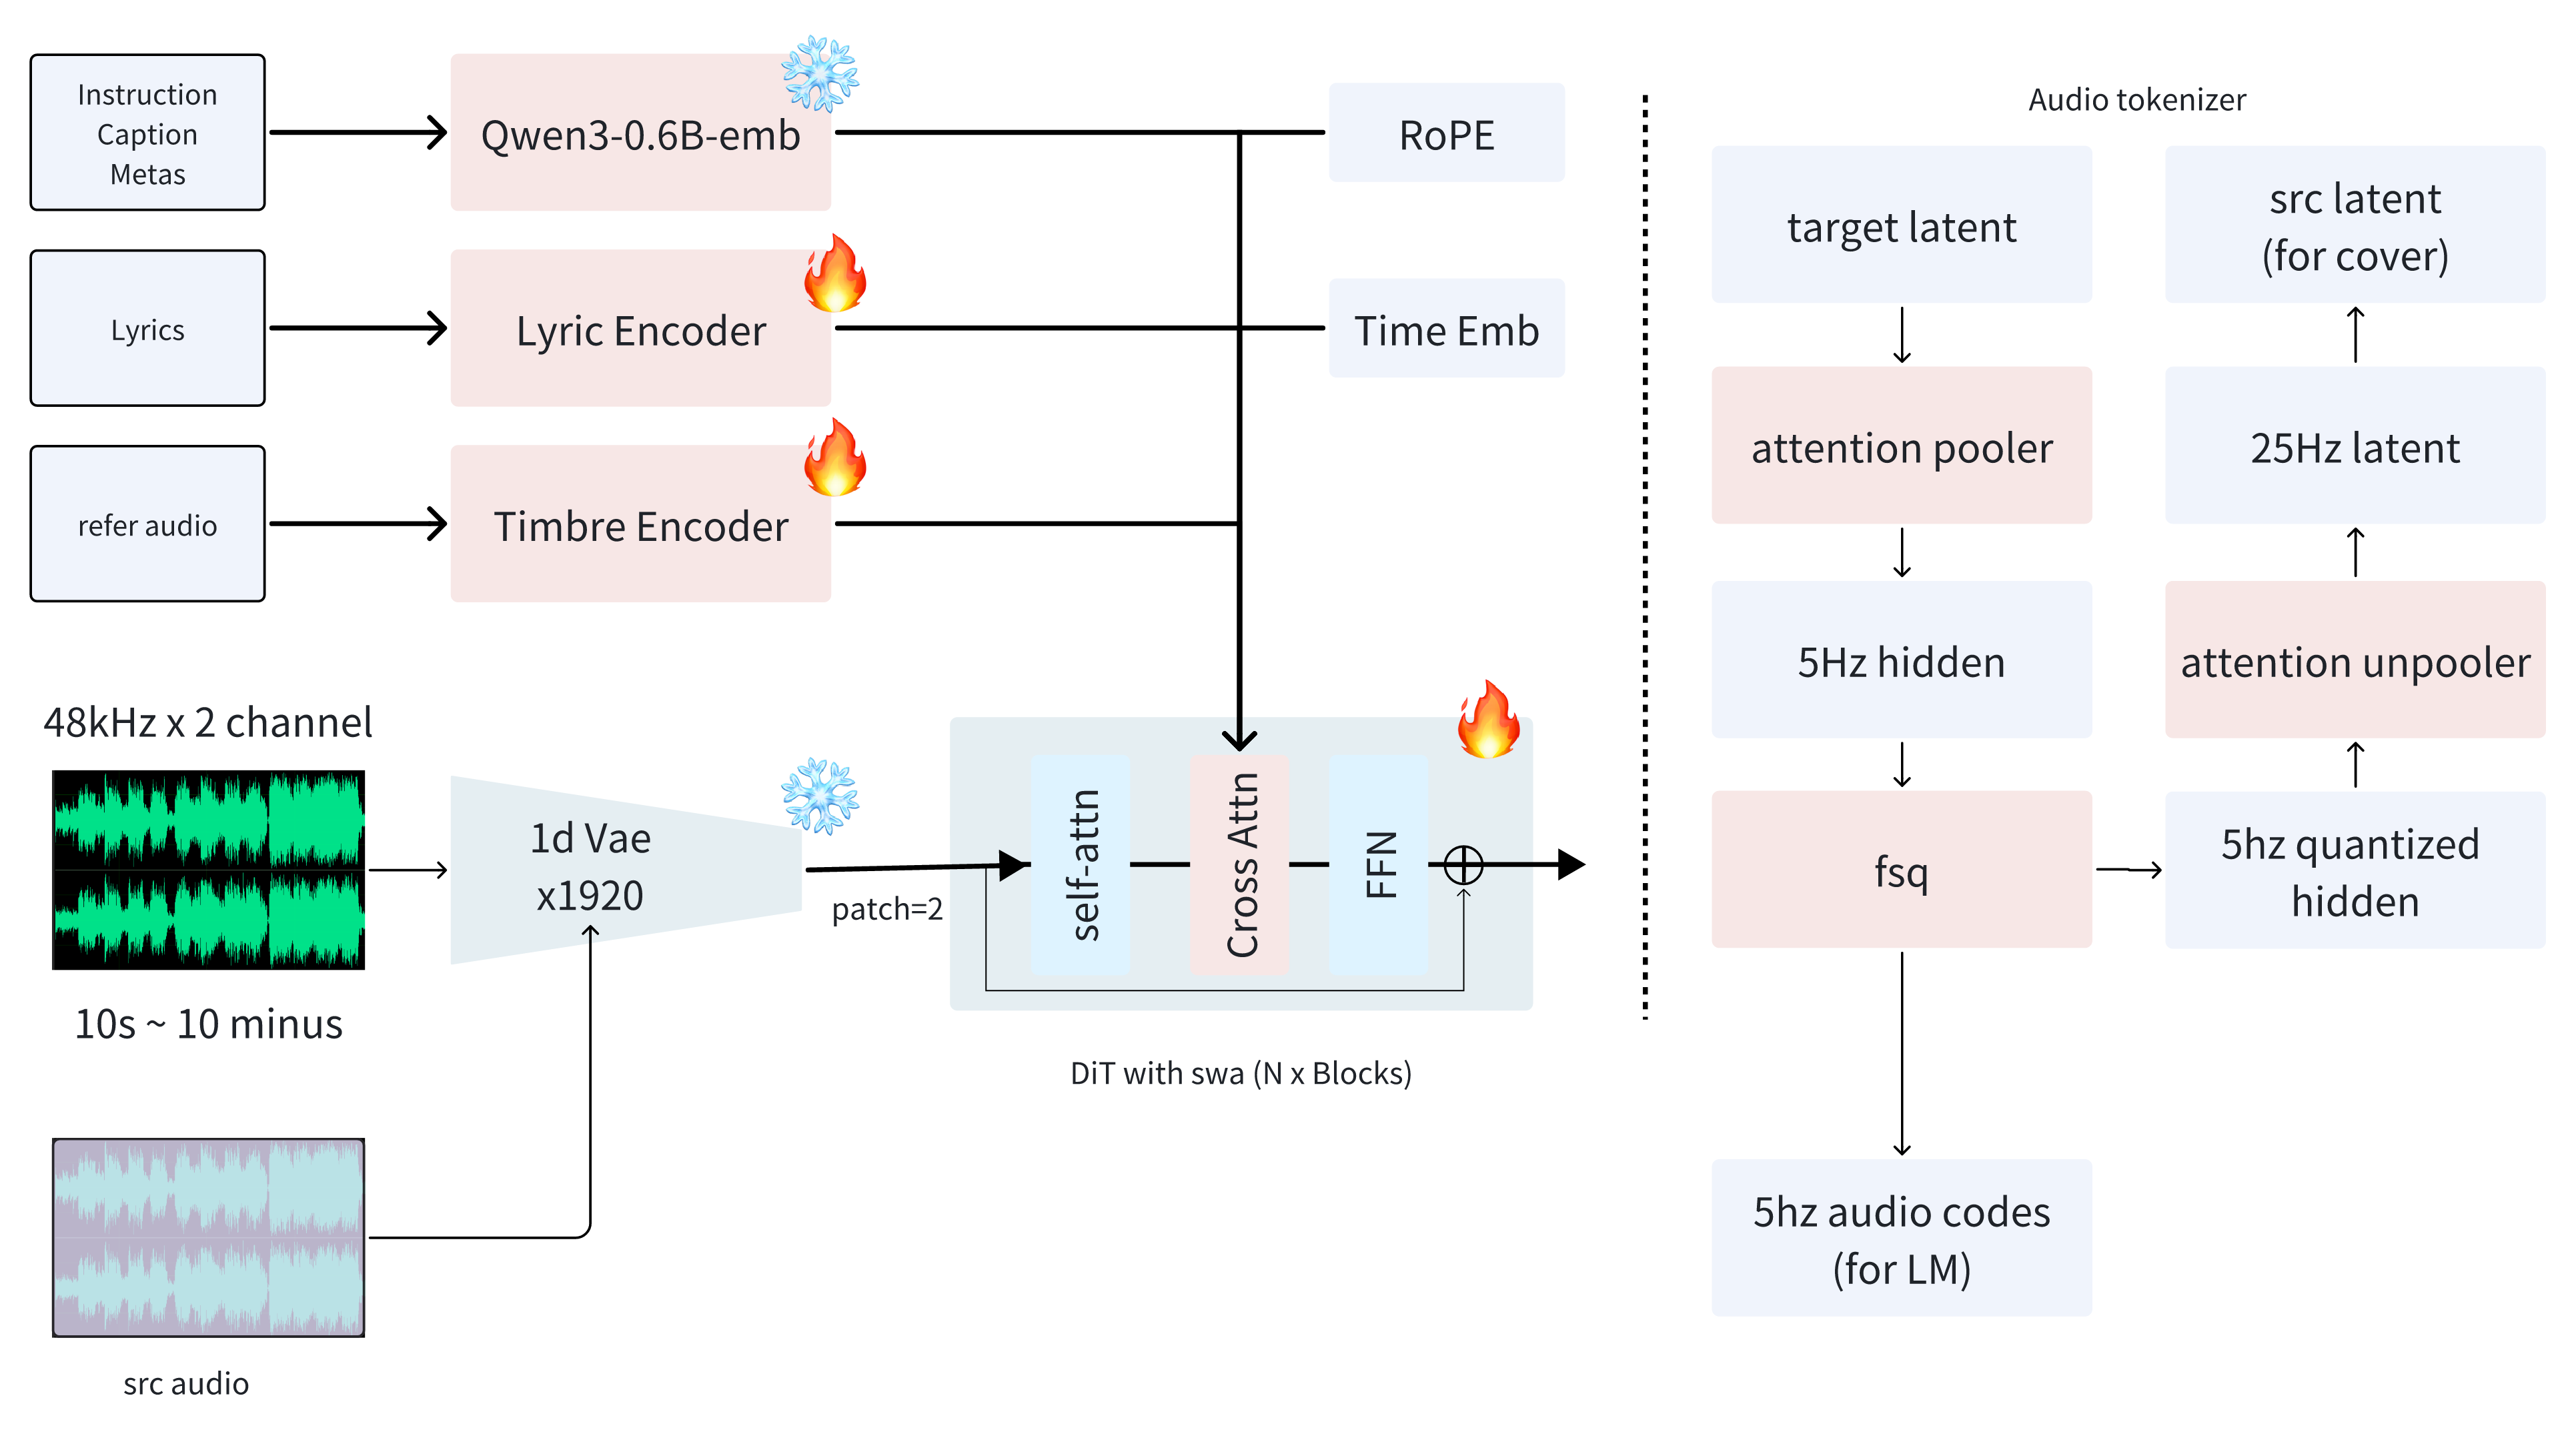
\includegraphics[width=\textwidth]{figures/ace-step-schema.png}
    \caption{Arquitectura de ACE-Step~1.5. Los bloques marcados con~\textit{snowflake} (Qwen3, VAE) permanecen congelados en todos los escenarios. Los marcados con~\textit{llama} son entrenables en fine-tuning completo. Con LoRA, \textbf{todo} el modelo queda congelado y solo se a\~naden matrices de bajo rango en \texttt{q\_proj}, \texttt{k\_proj}, \texttt{v\_proj} y \texttt{o\_proj} de la Cross~Attention del DiT.}
    \label{fig:ace-step-schema}
\end{figure}

El ajuste mediante \gls{lora} no modifica ninguno de los par\'ametros del modelo base; introduce matrices adicionales de bajo rango en las capas seleccionadas~\cite{hu2022lora}. Esto permite especializar el modelo en una tarea concreta, en este caso el control modal, con un coste de entrenamiento y almacenamiento mucho menor que un fine-tuning completo.

La hip\'otesis de trabajo es que, manteniendo congelado el grueso del conocimiento musical del modelo base, los adaptadores LoRA pueden aprender una se\~nal adicional asociada a modalidad. El equilibrio es delicado: una adaptaci\'on demasiado agresiva puede perjudicar musicalidad general, mientras que una adaptaci\'on demasiado suave puede no aportar separabilidad modal suficiente.

Desde el punto de vista del estado del arte en \textit{parameter-efficient fine-tuning}~\cite{ding2023peft}, esta hip\'otesis es coherente con el uso de LoRA en tareas donde se desea especializar comportamiento sin destruir capacidades generales del modelo base. En m\'usica, la dificultad adicional es que el objetivo no es solo sem\'antico, sino perceptivo y estructural en el tiempo.

En consecuencia, el criterio de ``\'exito'' no puede reducirse a una sola m\'etrica de clasificaci\'on: debe incorporar estabilidad temporal, consistencia modal por modo y validaci\'on auditiva de la salida generada.

\section{Los modos diat\'onicos}
\label{s:modos-diatonicos}

Para comprender el problema que aborda este trabajo, es necesario entender qu\'e es un modo musical y por qu\'e modos distintos producen sonoridades distintas, incluso cuando comparten exactamente las mismas notas.

\subsection{La escala de C mayor como referencia}

Una \textbf{escala musical} es una colecci\'on ordenada de notas separadas por distancias fijas. La distancia m\'inima entre dos notas consecutivas en el sistema occidental es el \textbf{semitono} (S); el doble de esa distancia es un \textbf{tono} (T).

A lo largo de esta memoria se utiliza la \textbf{nomenclatura anglosajona} para nombrar las notas, por coherencia con los \textit{prompts}, el c\'odigo del proyecto y la literatura de generaci\'on musical empleada. La equivalencia con la notaci\'on espa\~nola es la siguiente:

\begin{center}
\begin{tabular}{cccccccc}
\toprule
\textbf{Anglosajona} & C & D & E & F & G & A & B \\
\textbf{Espa\~nola}   & Do & Re & Mi & Fa & Sol & La & Si \\
\bottomrule
\end{tabular}
\end{center}

La escala de C mayor ---la m\'as familiar, equivalente a las teclas blancas del piano entre una C y la siguiente--- sigue el patr\'on:

\begin{center}
\large
\textbf{C} $\xrightarrow{\,T\,}$ \textbf{D} $\xrightarrow{\,T\,}$ \textbf{E} $\xrightarrow{\,S\,}$ \textbf{F} $\xrightarrow{\,T\,}$ \textbf{G} $\xrightarrow{\,T\,}$ \textbf{A} $\xrightarrow{\,T\,}$ \textbf{B} $\xrightarrow{\,S\,}$ \textbf{C}
\end{center}

La sucesi\'on \textbf{T--T--S--T--T--T--S} es la firma de la escala mayor: un patr\'on fijo de cinco tonos y dos semitonos (uno entre el 3.\textordmasculine\ y el 4.\textordmasculine\ grado, otro entre el 7.\textordmasculine\ y la octava) que define el car\'acter \emph{mayor}: brillante, estable y resolutivo.

La Figura~\ref{fig:teclado-c-mayor} ilustra este patr\'on sobre un teclado de piano. Las teclas negras ---que no forman parte de esta escala--- corresponden a los semitonos intermedios entre las blancas donde no hay tono completo.

\begin{figure}[htbp]
    \centering
    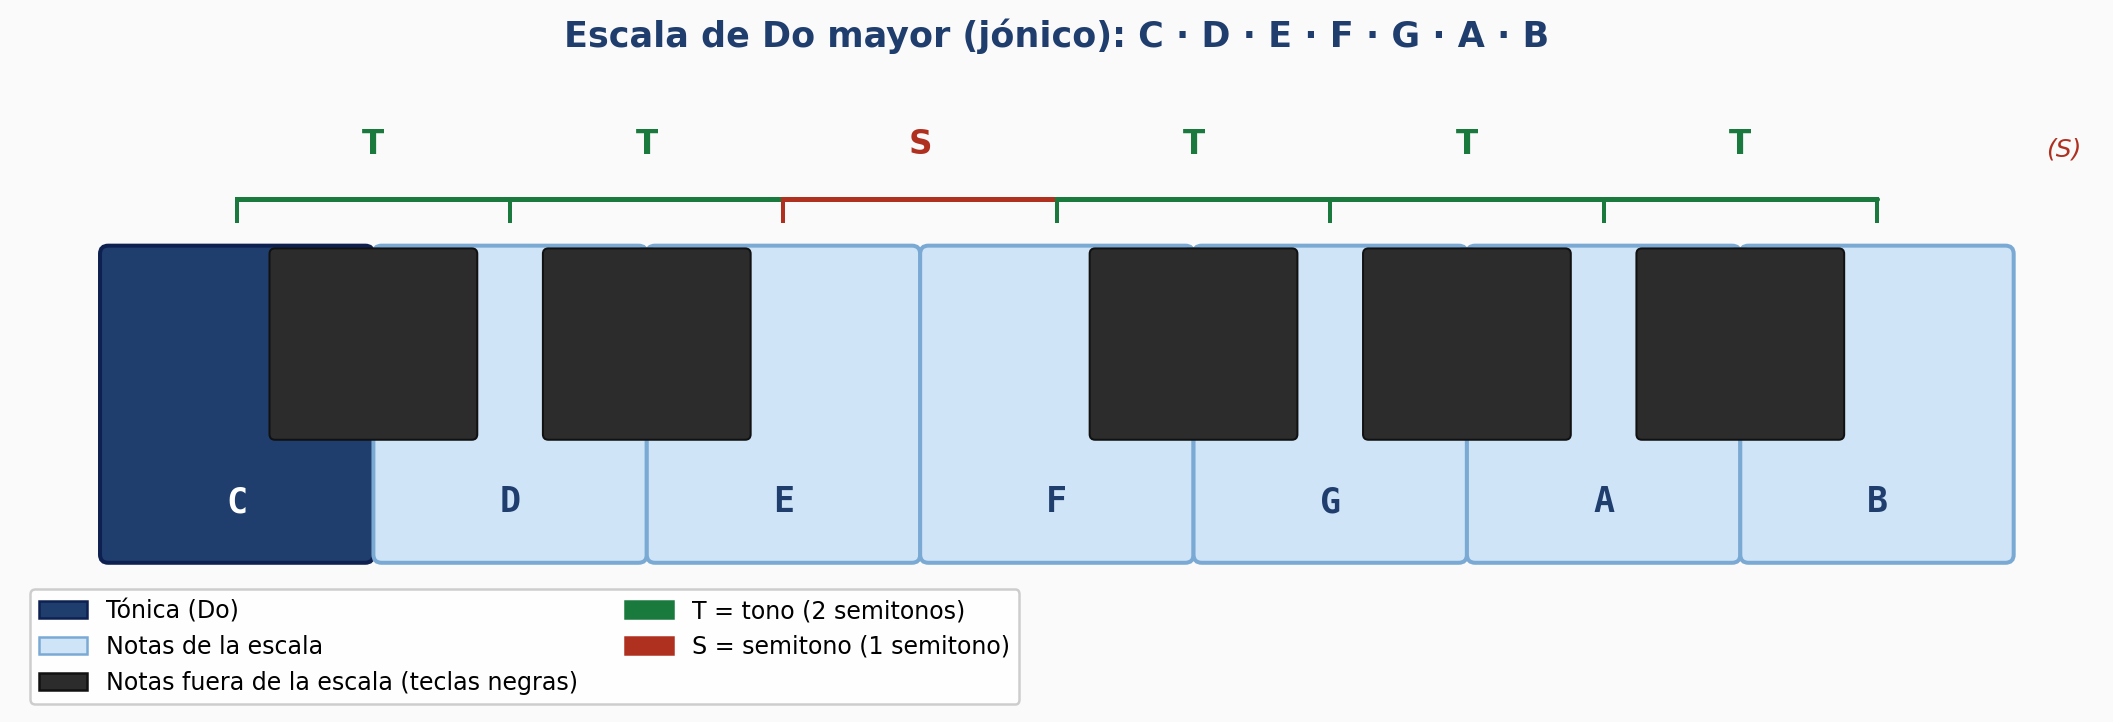
\includegraphics[width=\textwidth]{figures/modos_teclado_c_mayor.png}
    \caption{Escala de Do mayor sobre un teclado de piano. Las teclas azules son las siete notas de la escala; la tónica (Do) aparece en azul oscuro. Las marcas T (verde) y S (rojo) indican la distancia entre notas consecutivas de la escala.}
    \label{fig:teclado-c-mayor}
\end{figure}

\subsection{De la escala a los modos: mismo material, distinto punto de partida}

Los siete \textbf{modos diat\'onicos} se obtienen tomando las mismas siete notas de Do mayor, pero comenzando en cada una de ellas. Al cambiar el punto de partida, la t\'onica cambia, y con ella la distribuci\'on de tonos y semitonos respecto a esa nueva ra\'iz. Esto altera qu\'e intervalos caen sobre la nota de reposo y, por tanto, el car\'acter percibido de la m\'usica.

La Figura~\ref{fig:modos-grid} muestra los siete modos junto a su patr\'on de intervalos y su nota caracter\'istica ---la nota que distingue perceptivamente ese modo del jónico o del e\'olico y que define su color arm\'onico particular.

\begin{figure}[htbp]
    \centering
    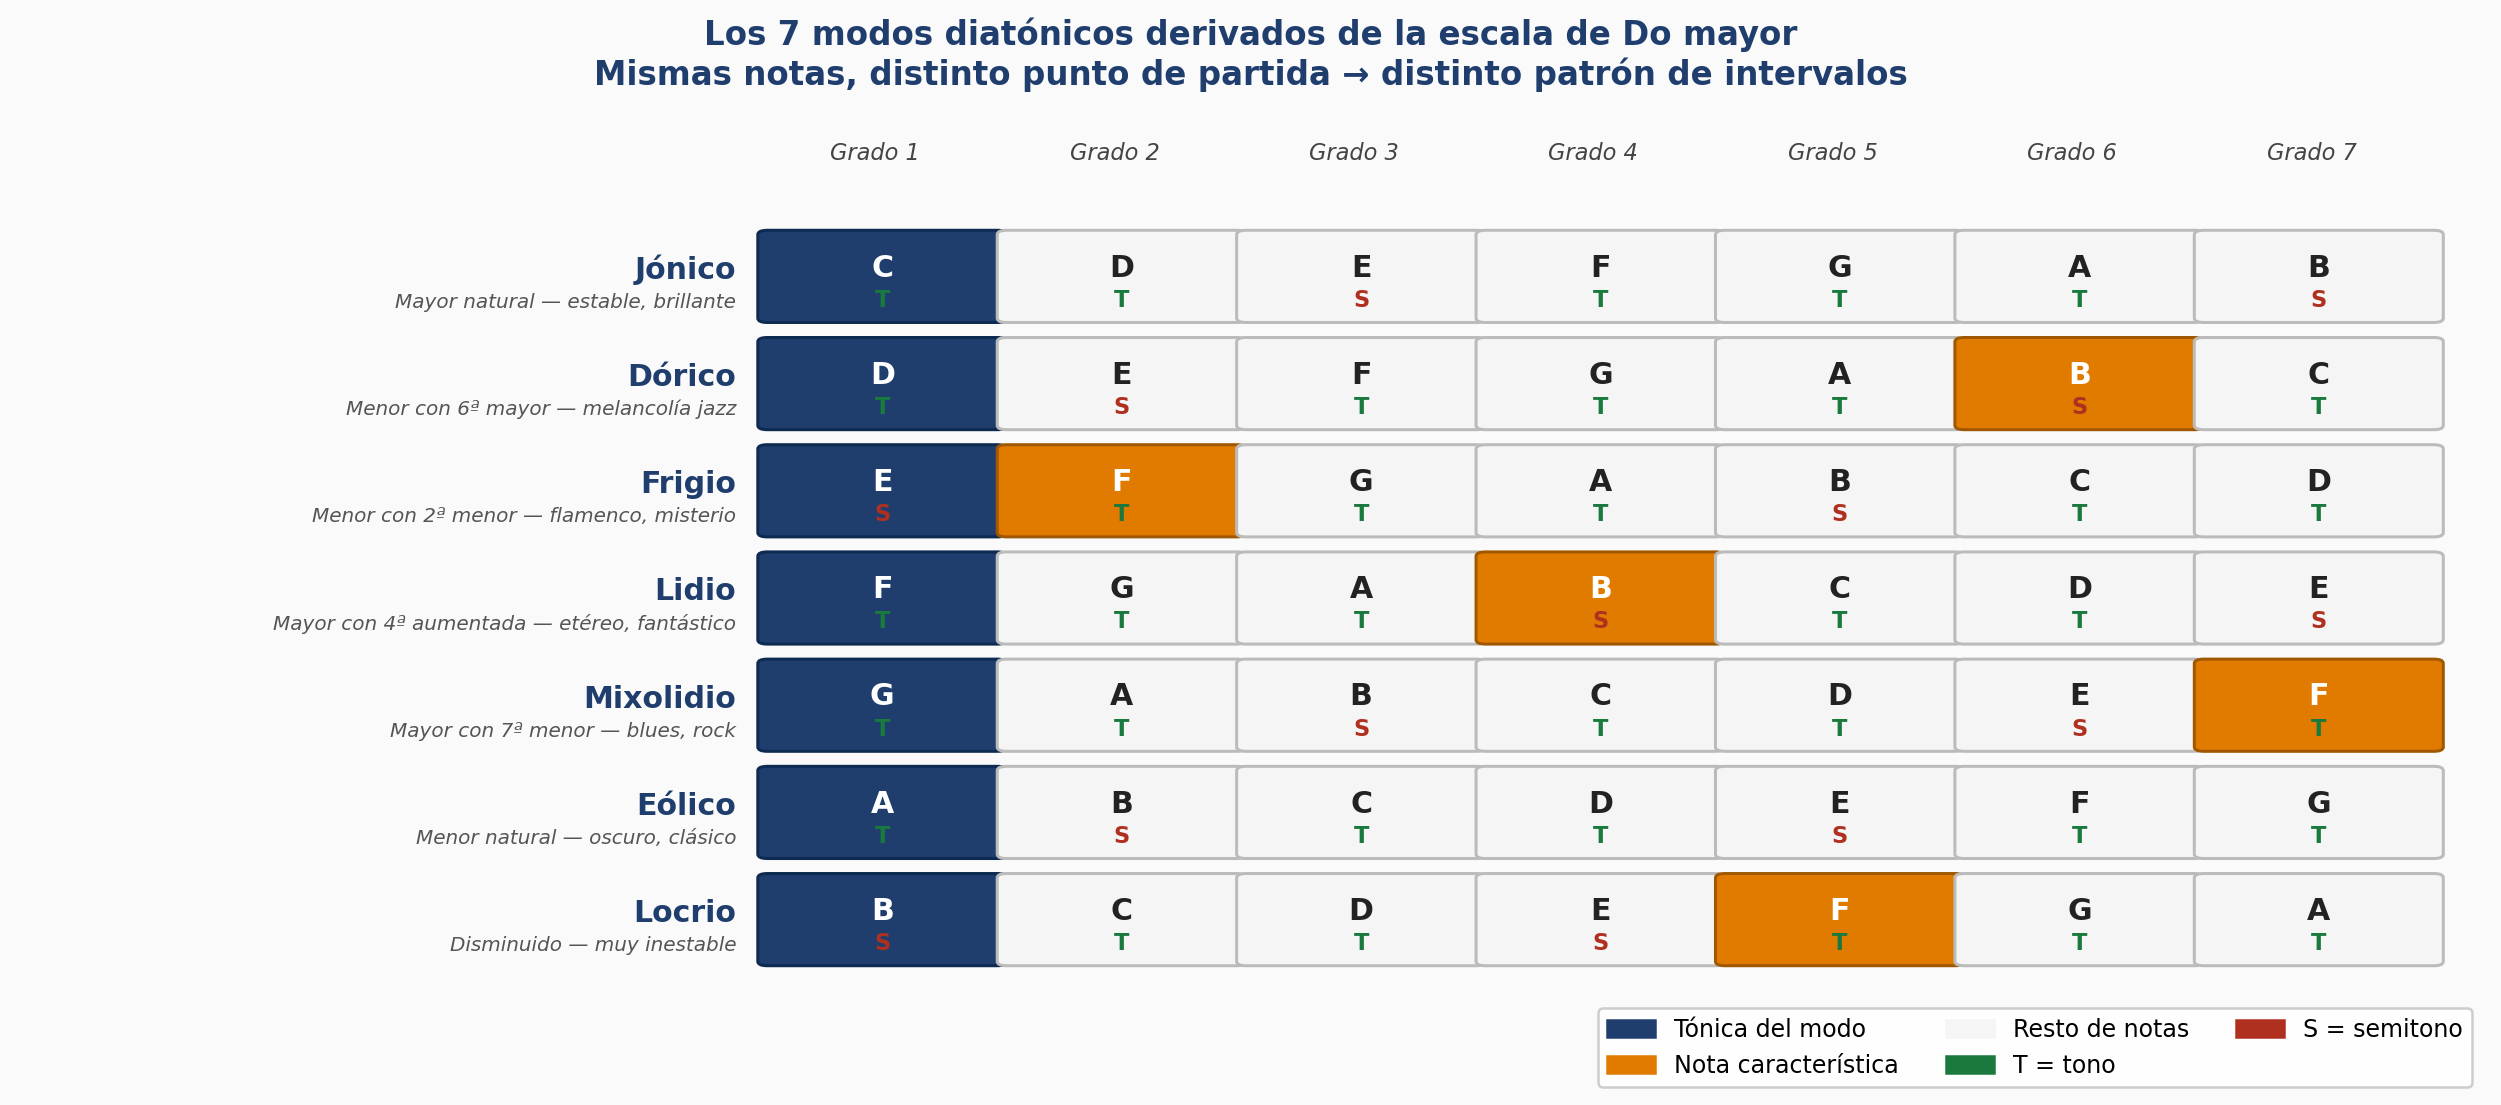
\includegraphics[width=\textwidth]{figures/modos_grid_intervalos.png}
    \caption{Los siete modos diat\'onicos derivados de la escala de Do mayor. Cada fila comienza en una nota distinta; el patr\'on T/S resultante cambia en cada modo. La celda naranja señala la nota caracter\'istica de cada modo, es decir, la nota que lo diferencia arm\'onicamente del mayor o del menor natural.}
    \label{fig:modos-grid}
\end{figure}

Los modos se dividen habitualmente en dos grandes grupos seg\'un su car\'acter:

\begin{itemize}
    \item \textbf{Modos mayores} (tienen 3\textordfeminine\ mayor sobre la t\'onica): j\'onico, lidio y mixolidio. Suenan brillantes y estables.
    \item \textbf{Modos menores} (tienen 3\textordfeminine\ menor sobre la t\'onica): d\'orico, frigio, e\'olico y locrio. Suenan m\'as oscuros o tensos.
\end{itemize}

La Tabla~\ref{tab:modos-ejemplos} sintetiza el car\'acter de cada modo, su nota caracter\'istica respecto al jónico, los géneros musicales donde aparece con mayor frecuencia y ejemplos de canciones populares que lo ilustran con claridad.

\begin{table}[htbp]
    \centering
    \caption{Caracterización de los siete modos diatónicos con ejemplos de música popular}
    \label{tab:modos-ejemplos}
    \small
    \begin{tabular}{llp{2.6cm}p{5.2cm}}
        \toprule
        \textbf{Modo} & \textbf{Car\'acter} & \textbf{G\'enero t\'ipico} & \textbf{Ejemplos} \\
        \midrule
        J\'onico
            & Brillante, estable
            & Pop, cl\'asico, folk
            & \textit{Imagine} (Lennon, 1971); \textit{Let It Be} (The Beatles, 1970) \\
        \addlinespace
        D\'orico
            & Melanc\'olico, con luminosidad
            & Jazz modal, soul, rock
            & \textit{So What} (Miles Davis, 1959); \textit{Oye Como Va} (Santana, 1970) \\
        \addlinespace
        Frigio
            & Oscuro, tenso, exótico
            & Flamenco, metal, m\'usica \'arabe
            & Bulerias y soleá flamencas; \textit{Wherever I May Roam} (Metallica, 1991) \\
        \addlinespace
        Lidio
            & Et\'ereo, flotante, onírico
            & M\'usica de cine, jazz
            & Tema de apertura de \textit{Los Simpsons} (Elfman, 1989); \textit{Flying} (The Beatles, 1967) \\
        \addlinespace
        Mixolidio
            & Mayor con tensión, bluesy
            & Blues, rock, celta
            & \textit{Norwegian Wood} (The Beatles, 1965); \textit{Gloria} (Van Morrison, 1964) \\
        \addlinespace
        E\'olico
            & Oscuro, introspectivo
            & Rock, pop, cl\'asico
            & \textit{All Along the Watchtower} (Dylan, 1967); \textit{Losing My Religion} (R.E.M., 1991) \\
        \addlinespace
        Locrio
            & Inestable, disonante
            & Metal progresivo, jazz avanzado
            & Muy raro en m\'usica popular; aparece en algunos pasajes de metal y jazz moderno \\
        \bottomrule
    \end{tabular}
\end{table}

La escasez de ejemplos populares de locrio ilustra de forma directa por qu\'e ese modo es el m\'as dif\'icil de controlar: su tr\'itono sobre la t\'onica genera una inestabilidad tan acusada que la m\'usica tiende a resolver hacia otro centro tonal. Esta misma dificultad se refleja en los resultados experimentales de este trabajo, donde locrio es el modo con peor puntuaci\'on en evaluaci\'on manual (Secci\'on~\ref{s:analisis-modos-ref}).

\subsection{Por qu\'e una sola nota cambia el car\'acter: el ejemplo d\'orico}

El caso m\'as ilustrativo de c\'omo una diferencia m\'inima produce un efecto radical es la comparaci\'on entre el modo e\'olico (menor natural) y el modo d\'orico. Ambos son modos menores que comparten seis de sus siete notas; la \'unica diferencia es la sexta escalar:

\begin{itemize}
    \item \textbf{Re e\'olico:} D -- E -- F -- G -- A -- \textbf{Bb} -- C \quad (6\textordfeminine\ menor = Si bemol)
    \item \textbf{Re d\'orico:} D -- E -- F -- G -- A -- \textbf{B} -- C \quad (6\textordfeminine\ mayor = Si)
\end{itemize}

Esa \'unica nota ---Si bemol frente a Si natural--- es suficiente para transformar una sonoridad oscura y cl\'asica (e\'olico) en una sonoridad melanc\'olica con un punto de luminosidad (d\'orico), caracter\'istica del jazz modal y del soul. Canciones como \emph{So What} de Miles Davis o \emph{Scarborough Fair} son ejemplos conocidos del modo d\'orico.

La Figura~\ref{fig:comparativa-ionico-dorico} ilustra c\'omo, partiendo de las mismas notas de Do mayor, el modo j\'onico (raíz en Do) y el modo d\'orico (ra\'iz en Re) generan patrones de intervalos completamente distintos sobre sus respectivas t\'onicas.

\begin{figure}[htbp]
    \centering
    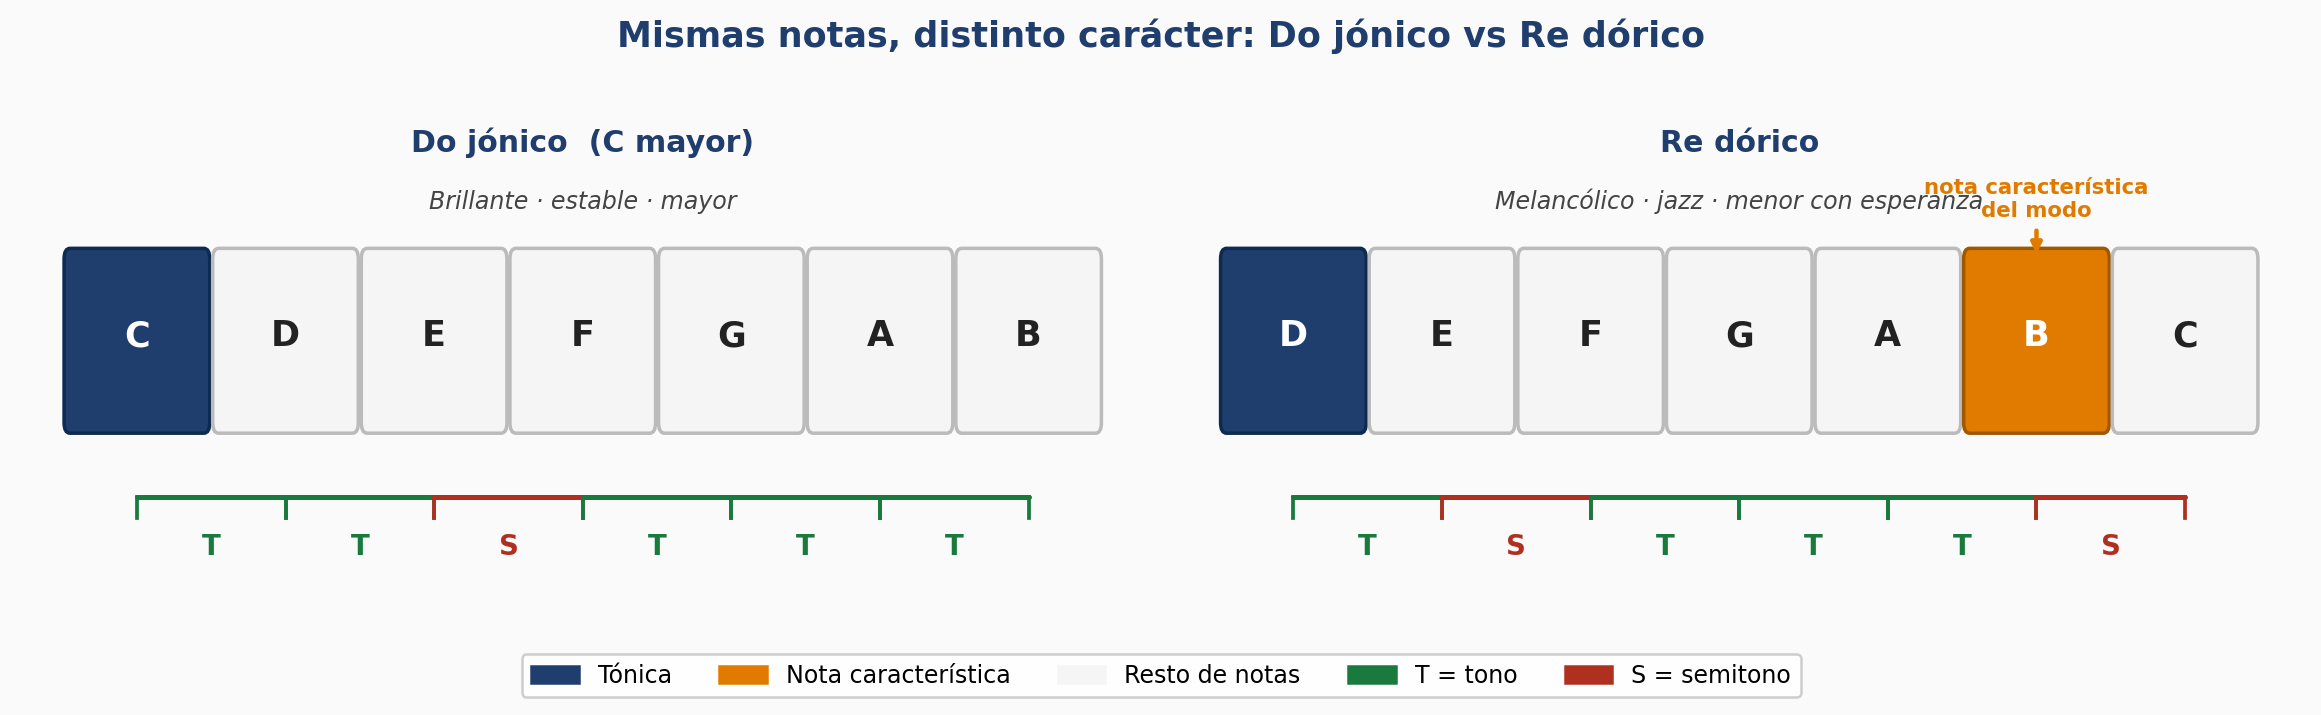
\includegraphics[width=\textwidth]{figures/modos_comparativa_ionico_dorico.png}
    \caption{Comparativa entre Do j\'onico y Re d\'orico. Ambos modos utilizan exactamente las mismas siete notas (las teclas blancas del piano), pero al tomar Ra\'iz distinta, el patr\'on de intervalos cambia: el semitono cae en distinto lugar sobre la t\'onica, lo que determina el car\'acter del modo. La nota caracter\'istica del d\'orico (Si, naranja) es la que lo distingue del menor natural.}
    \label{fig:comparativa-ionico-dorico}
\end{figure}

\subsection{Implicaciones para la generaci\'on autom\'atica de m\'usica}

Este an\'alisis tiene una consecuencia directa para el problema que aborda el presente trabajo. Un modelo generativo que aprende a producir m\'usica a partir de grandes vol\'umenes de datos tiende a reflejar los sesgos de esa distribuci\'on. Dado que la m\'usica popular est\'a dominada por modos mayores y por el menor natural (e\'olico), el modelo base tendr\'a un sesgo hacia esas sonoridades.

Cuando se le pide que genere en modo d\'orico, el modelo puede producir una pieza en Re menor ignorando la sexta mayor ---una diferencia de un solo semitono que pasa desapercibida si no se escucha con atenci\'on, pero que elimina el car\'acter espec\'ificamente d\'orico. Este es precisamente el tipo de error sistem\'atico que se observa en la evaluaci\'on manual del presente trabajo (Secci\'on~\ref{s:confusion-mayor-menor}), y la raz\'on por la que el control modal es un reto m\'as sutil de lo que aparenta.

\section{Control modal y dificultad del problema}

Imponer modalidad de forma robusta implica controlar el centro tonal, el color modal y la estabilidad arm\'onica en el tiempo. En la pr\'actica, esto es m\'as exigente que generar audio plausible, porque requiere mantener coherencia musical global y diferenciaci\'on entre modos cercanos, especialmente en contextos con progresiones ambiguas.

Adem\'as, la modalidad es una propiedad dif\'icil de medir de forma autom\'atica: un oyente puede percibir claramente el car\'acter modal de una pieza aunque la t\'onica no se afirme con fuerza en cada instante. Por eso una evaluaci\'on fiable necesita combinar m\'etricas autom\'aticas, que dan una se\~nal cuantitativa pero parcial, con escucha humana estructurada que confirme el color modal real.

\section{S\'intesis del estado de la cuesti\'on y hueco identificado}

Del an\'alisis anterior se desprende un hueco claro: existen modelos capaces de generar m\'usica de calidad, y existen t\'ecnicas eficientes de adaptaci\'on como LoRA, pero faltan protocolos pr\'acticos y reproducibles para validar control modal fino en escenarios de coste moderado. Este trabajo se posiciona en ese hueco, proponiendo una metodolog\'ia experimental replicable que combina evaluaci\'on autom\'atica, evaluaci\'on musical informada y trazabilidad de decisiones experimentales.

Adicionalmente, el desarrollo del proyecto ha requerido intervenir directamente sobre los ficheros de entrenamiento de ACE-Step para corregir incidencias detectadas durante la experimentaci\'on (problemas de carga de adaptadores, comportamiento inconsistente en \texttt{save\_every\_n\_epochs}, errores de orquestaci\'on en inferencia por lotes). Estas correcciones fueron necesarias para garantizar la validez de los experimentos posteriores y se documentan en el cap\'itulo de metodolog\'ia.

\section{Posicionamiento del trabajo respecto al estado actual}

La Tabla~\ref{tab:posicionamiento-trabajo} resume el posicionamiento de este \gls{pfg} frente a enfoques habituales en generaci\'on musical condicionada.

\begin{table}[htbp]
    \centering
    \caption{Posicionamiento del trabajo respecto a enfoques habituales}
    \label{tab:posicionamiento-trabajo}
    \begin{tabular}{lp{4.2cm}p{4.2cm}}
        \toprule
        \textbf{Dimensi\'on} & \textbf{Enfoque habitual} & \textbf{Enfoque en este trabajo} \\
        \midrule
        Adaptaci\'on del modelo & Fine-tuning amplio o no controlado & LoRA focalizado y conservador \\
        Objetivo principal & Calidad perceptiva general & Calidad + control modal expl\'icito \\
        Evaluaci\'on & Predominio de m\'etrica autom\'atica & Pipeline dual: autom\'atica + escucha informada \\
        Selecci\'on experimental & Iteraci\'on poco trazable & Ranking determinista de checkpoints \\
        Coste computacional & Alto o variable & Acotado y compatible con iteraci\'on acad\'emica \\
        \bottomrule
    \end{tabular}
\end{table}

En s\'intesis, el estado de la cuesti\'on justifica una estrategia experimental centrada en trazabilidad, control de sesgos y validaci\'on dual. Este enfoque marca la transici\'on natural hacia la metodolog\'ia empleada en el proyecto.

\chapter{Metodolog\'ia}
\label{ch:metodologia}

\section{Entorno y recursos}

El trabajo se distribuy\'o entre dos entornos: el ordenador personal del autor y una m\'aquina remota con GPU proporcionada por el tutor a trav\'es de la universidad. Esta separaci\'on no fue una elecci\'on metodol\'ogica sino una necesidad: el equipo local no dispone de GPU suficiente para entrenar modelos generativos de este tama\~no, por lo que la totalidad del entrenamiento y la inferencia se ejecut\'o en remoto.

\textbf{M\'aquina local.} Ordenador personal utilizado para el desarrollo de scripts, edici\'on de la memoria, an\'alisis de resultados, escucha de audios generados y visualizaci\'on de figuras.

\textbf{M\'aquina remota (GPU).} Servidor Linux con GPU NVIDIA, accesible a trav\'es de la red universitaria, sobre el que se ejecutaron los entrenamientos LoRA y la inferencia por lotes. Se emplearon las siguientes herramientas de acceso remoto, cuyo uso no hab\'ia formado parte del plan de estudios previo y fue necesario aprender durante el proyecto:

\begin{itemize}
    \item \textbf{PuTTY.} Cliente SSH para Windows que permite abrir terminales en la m\'aquina remota. Se utiliz\'o para lanzar entrenamientos, ejecutar scripts de inferencia y monitorizar el progreso de los experimentos en tiempo real.
    \item \textbf{WinSCP.} Programa para transferir ficheros entre el equipo local y el servidor a trav\'es de SFTP (un protocolo de transferencia de ficheros sobre SSH). Se emple\'o para enviar scripts, datasets preprocesados y configuraciones al servidor, y para descargar los resultados (CSV de m\'etricas, audios generados, figuras) al equipo local para su an\'alisis.
    \item \textbf{T\'unel SSH.} Mediante reenv\'io de puertos (\textit{port forwarding}) por SSH, se expusieron localmente la interfaz Gradio y la API REST del servidor. Esto permiti\'o interactuar con el modelo desde el navegador del equipo local sin necesidad de abrir puertos en el cortafuegos universitario.
\end{itemize}

Este flujo de trabajo---desarrollo local, ejecuci\'on remota, descarga de resultados---es el habitual en investigaci\'on con modelos de aprendizaje profundo y requiri\'o familiarizarse con herramientas y conceptos de administraci\'on de sistemas que complementaron la formaci\'on acad\'emica recibida.

El flujo experimental completo incluy\'o: preparaci\'on de datos, preprocesado a tensores, entrenamiento LoRA, inferencia por lotes y evaluaci\'on manual asistida por scripts.

\section{Construcci\'on del dataset}

Se construy\'o un dataset de 102 clips de audio de entre 20 y 50 segundos. Los fragmentos se obtuvieron a partir de canciones existentes y fueron recortados manualmente para conservar secciones representativas a nivel arm\'onico. La selecci\'on de canciones y la comprensi\'on del car\'acter perceptivo de cada modo se apoyaron, entre otros recursos, en el canal de divulgaci\'on musical \textit{David Bennett Piano}\footnote{Canal de YouTube \textit{David Bennett Piano}: \url{https://www.youtube.com/@davidbennettpiano}\linebreak (consultado en 2025--2026). El canal ofrece an\'alisis audio-musicales accesibles sobre modos diat\'onicos y su uso en m\'usica popular, lo que facilit\'o la identificaci\'on de ejemplos representativos para cada modo.}, cuyo enfoque did\'actico sobre los modos en m\'usica popular result\'o especialmente \'util para identificar ejemplos con car\'acter modal claro y verificable.

Distribuci\'on por modo:

\begin{table}[htbp]
    \centering
    \caption{Distribuci\'on de clips por modo en el dataset}
    \begin{tabular}{lr}
        \toprule
        \textbf{Modo} & \textbf{N\'umero de clips} \\
        \midrule
        J\'onico & 7 \\
        D\'orico & 21 \\
        Frigio & 16 \\
        Lidio & 18 \\
        Mixolidio & 18 \\
        E\'olico & 14 \\
        Locrio & 8 \\
        \bottomrule
    \end{tabular}
\end{table}

El reparto por modo no es uniforme y responde a dos decisiones deliberadas. En primer lugar, el modo j\'onico aparece deliberadamente infrarrepresentado: la m\'usica occidental ---y por extensi\'on, la mayor parte del corpus de entrenamiento original del modelo base--- es predominantemente j\'onica, por lo que se entendi\'o que era preferible reservar la capacidad de adaptaci\'on del LoRA para los modos minoritarios. Los resultados confirman esta intuici\'on: el modo j\'onico obtiene de las mejores puntuaciones en evaluaci\'on manual a pesar de contar con solo 7 clips, lo que sugiere que un n\'umero peque\~no de ejemplos bien seleccionados es suficiente cuando el modelo base ya conoce bien la sonoridad. En el extremo contrario, el modo locrio fue el m\'as dif\'icil de representar: encontrar ejemplos claros y musicalmente significativos en m\'usica popular result\'o muy complicado debido a su rareza estil\'istica, lo que constituye una limitaci\'on conocida para el entrenamiento de ese modo.

\section{Entrenamiento LoRA}

La l\'inea experimental principal utiliza ACE-Step 1.5 y adaptadores LoRA con configuraciones exploradas por rejilla de hiperpar\'ametros. La configuraci\'on m\'as prometedora de la fase exploratoria inicial fue:

\begin{itemize}
    \item rank = 64
    \item alpha = 128
    \item dropout = 0.05
    \item learning rate = $5 \cdot 10^{-5}$
    \item checkpoint de referencia: epoch 100
\end{itemize}

Con el fin de no degradar capacidades generales del modelo base, se utiliz\'o una estrategia de etiquetado conservadora en los captions de entrenamiento, centrada en el modo objetivo y evitando fijar estilo, tempo o instrumentaci\'on de forma r\'igida.

La configuraci\'on de referencia del estudio (run\_D) se ejecut\'o con los par\'ametros detallados en la Tabla~\ref{tab:run-d-config} y ha sido completamente evaluada tanto de forma autom\'atica como mediante escucha informada.

\subsection{Interfaz de entrenamiento y par\'ametros configurables}
\label{ss:ui-training}

ACE-Step 1.5 incorpora una interfaz gr\'afica Gradio con una pesta\~na de entrenamiento LoRA que permite configurar todos los par\'ametros sin necesidad de editar c\'odigo. La Figura~\ref{fig:interfaz-lora} muestra esta interfaz tal y como se utiliz\'o durante el proyecto.

\begin{figure}[htbp]
    \centering
    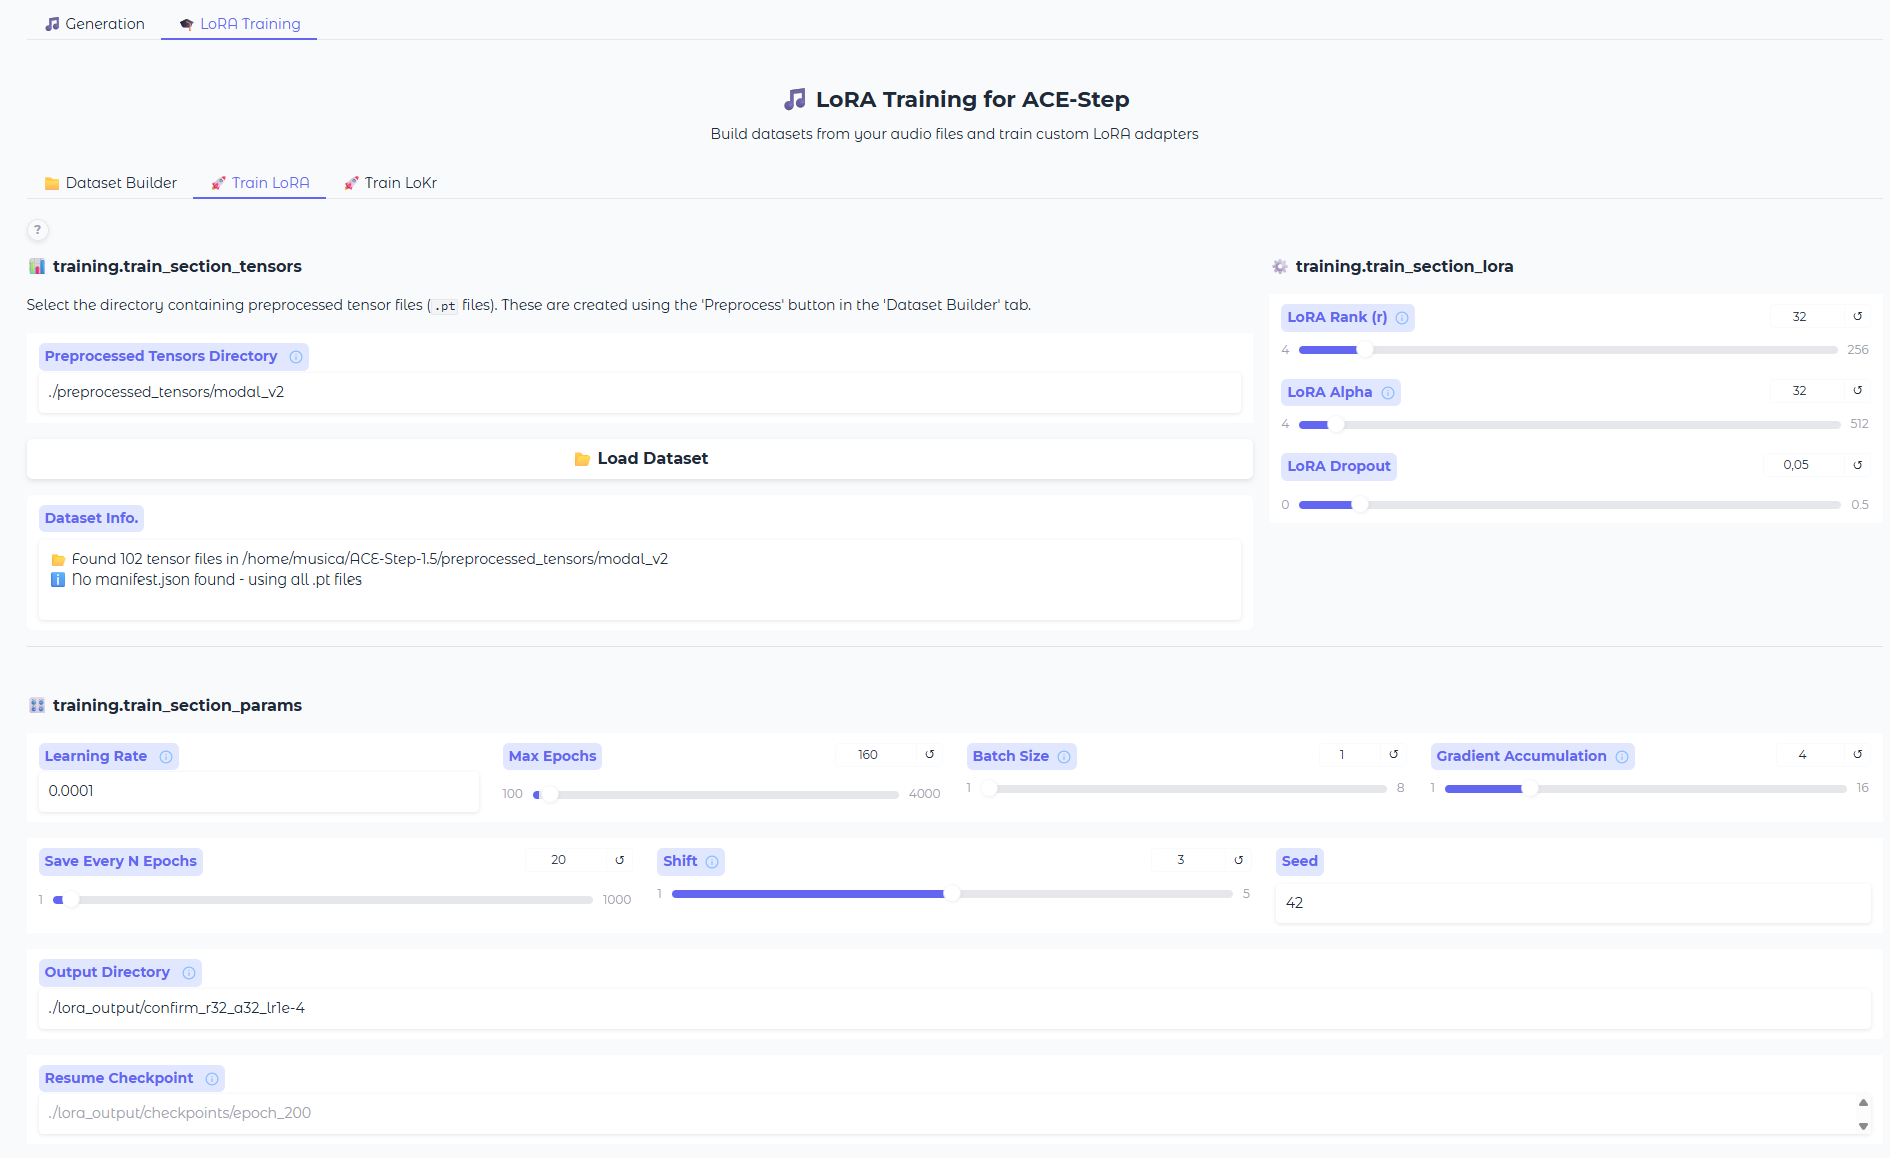
\includegraphics[width=\textwidth]{figures/interfaz_lora.png}
    \caption{Interfaz de entrenamiento LoRA de ACE-Step~1.5. Los paneles permiten seleccionar el dataset de tensores, configurar los hiperpar\'ametros LoRA y los par\'ametros generales del entrenamiento, y especificar el directorio de salida de checkpoints.}
    \label{fig:interfaz-lora}
\end{figure}

La interfaz organiza los par\'ametros en tres grupos. La Tabla~\ref{tab:params-ui} describe cada uno, su significado y su efecto sobre el entrenamiento.

\begin{table}[htbp]
    \centering
    \caption{Par\'ametros configurables en la interfaz de entrenamiento LoRA}
    \label{tab:params-ui}
    \small
    \begin{tabular}{lp{3.8cm}p{5cm}}
        \toprule
        \textbf{Par\'ametro} & \textbf{Significado} & \textbf{Efecto en el entrenamiento} \\
        \midrule
        \multicolumn{3}{l}{\textit{Par\'ametros LoRA}} \\
        \midrule
        Rank ($r$) & Dimensi\'on de las matrices de bajo rango $A$ y $B$ & Mayor rango = m\'as par\'ametros entrenables = m\'as capacidad de adaptaci\'on, pero mayor coste de memoria y riesgo de sobreentrenamiento \\
        Alpha ($\alpha$) & Factor de escala del adaptador (ver Ec.~\ref{eq:lora}) & Controla la magnitud de la actualizaci\'on LoRA; cuando $\alpha = r$ la escala es neutra (1.0) \\
        Dropout & Probabilidad de desactivar activaciones LoRA durante entrenamiento & Regularizaci\'on: valores altos reducen sobreajuste pero enlentecen la convergencia \\
        \midrule
        \multicolumn{3}{l}{\textit{Par\'ametros de entrenamiento}} \\
        \midrule
        Learning rate & Tama\~no del paso en el descenso de gradiente & Valor cr\'itico: demasiado alto produce inestabilidad, demasiado bajo convergencia lenta \\
        Max epochs & N\'umero m\'aximo de \'epocas completas sobre el dataset & Determina la duraci\'on m\'axima; el checkpoint \'optimo suele estar antes del final \\
        Batch size & Muestras procesadas por paso de gradiente & Limitado por VRAM; valores bajos aumentan el ruido del gradiente pero permiten mayor variabilidad \\
        Gradient accumulation & N\'umero de pasos acumulados antes de actualizar pesos & El batch efectivo real es $\text{batch\_size} \times \text{acumulaci\'on}$; permite simular batches mayores sin coste de memoria adicional \\
        Save every $N$ epochs & Frecuencia de guardado de checkpoints intermedios & Frecuencia alta permite analizar la curva de convergencia y seleccionar el checkpoint \'optimo \\
        Shift & Par\'ametro de la distribuci\'on lognormal de muestreo de timesteps & Valores altos priorizan timesteps con mayor ruido (etapas iniciales del flujo), modificando qu\'e aspectos del audio aprende a reconstruir el modelo \\
        Seed & Semilla aleatoria & Garantiza reproducibilidad del entrenamiento \\
        \bottomrule
    \end{tabular}
\end{table}

En este estudio, el batch efectivo fue siempre $1 \times 4 = 4$ muestras (batch size~=~1 con acumulaci\'on de gradiente~=~4), y se guard\'o un checkpoint cada 20 \'epocas para permitir la selecci\'on del mejor punto de convergencia mediante evaluaci\'on auditiva posterior.

\subsection{Qu\'e se congela con LoRA y funci\'on de p\'erdida}
\label{ss:lora-freeze-loss}

En un fine-tuning LoRA, \textbf{todos los par\'ametros del modelo base quedan congelados}. En lugar de modificar directamente los pesos~$W$ de las capas objetivo, se a\~nade una rama paralela de bajo rango:

\begin{equation}
    W' = W + \frac{\alpha}{r}\,BA
    \label{eq:lora}
\end{equation}

donde $W \in \mathbb{R}^{d \times k}$ son los pesos originales congelados, $B \in \mathbb{R}^{d \times r}$ y $A \in \mathbb{R}^{r \times k}$ son las matrices LoRA entrenables, $r$ es el rango y $\alpha$ el factor de escala. Solo $A$ y $B$ reciben gradiente; el resto del modelo no.

En este trabajo, los m\'odulos objetivo son \texttt{q\_proj}, \texttt{k\_proj}, \texttt{v\_proj} y \texttt{o\_proj} de los bloques Cross~Attention del DiT, es decir, las proyecciones de query, key, value y output de la atenci\'on que conecta el texto condicionante con el latente de audio. El n\'umero de par\'ametros entrenables es del orden de $2 \times r \times (d + k) \times N_\text{bloques}$, representando menos del 1\,\% del total del modelo.

ACE-Step utiliza \textit{flow matching}~\cite{lipman2023flow} como objetivo de entrenamiento, un marco emparentado con los modelos de difusi\'on cl\'asicos~\cite{ho2020ddpm}. La idea, en t\'erminos sencillos, es la siguiente: durante el entrenamiento se parte del latente limpio $z_1$ (la representaci\'on del audio real) y se mezcla con ruido $z_0$ en una proporci\'on intermedia $t$, obteniendo un latente parcialmente ruidoso $z_t$. Al modelo se le pide que, observando $z_t$, prediga la \emph{direcci\'on de limpieza}: el vector $(z_1 - z_0)$ que llevar\'ia del ruido al audio. La p\'erdida mide cu\'anto se parece la predicci\'on del modelo a esa direcci\'on real, mediante el error cuadr\'atico medio entre ambos vectores:

\begin{equation}
    \mathcal{L} = \mathbb{E}_{t,\,z_0,\,z_1}\bigl[\|v_\theta(z_t,\,t,\,c) - (z_1 - z_0)\|^2\bigr]
    \label{eq:flow-loss}
\end{equation}

donde $v_\theta$ es la predicci\'on del modelo y $c$ es el embedding del texto condicionante. El valor $t$ se muestrea de una distribuci\'on lognormal con $\mu=-0.4$ y $\sigma=1.0$, lo que concentra el entrenamiento en niveles de ruido intermedios, donde la se\~nal de aprendizaje es m\'as informativa que en los extremos (ni ruido puro ni audio ya limpio).

\subsection{Flujo de entrenamiento con ejemplo}
\label{ss:training-flow}

Para una muestra de entrenamiento con prompt \textit{``dorian mode, jazz-fusion instrumental, D dorian...''} y su clip de audio correspondiente, el flujo es:

\begin{enumerate}
    \item El audio (48\,kHz) pasa por el VAE congelado y se obtiene el latente limpio $z_1$.
    \item Se muestrea $t$ y ruido $z_0$; se calcula el latente ruidoso $z_t = (1-t)z_0 + t\,z_1$.
    \item El prompt pasa por el encoder Qwen3 congelado y genera el embedding $c$.
    \item El DiT (con adaptadores LoRA activos) predice $v_\theta(z_t, t, c)$.
    \item Se calcula la p\'erdida seg\'un la Ecuaci\'on~\ref{eq:flow-loss}.
    \item El gradiente actualiza \textbf{\'unicamente} las matrices LoRA $A$ y $B$ de cada capa objetivo.
\end{enumerate}

\subsection{Trayectoria experimental y selecci\'on de hiperpar\'ametros}
\label{ss:training-curves}

El trabajo experimental sigui\'o una progresi\'on en tres fases sucesivas, cada una informada por los resultados de la anterior.

\textbf{Fase exploratoria inicial.} Se realizaron entrenamientos largos (del orden de 5\,000 \'epocas) con guardado de checkpoint cada 200 \'epocas. La escucha de los audios revel\'o que a partir de la \'epoca 400 el modelo se encontraba claramente sobreentrenado: el audio dejaba de ser musicalmente legible. Esta fase, aunque no produjo configuraciones definitivas, fue clave para acotar el rango \'util de \'epocas y descartar el uso exclusivo de la loss como criterio de parada.

\textbf{Fase de afinado y configuraci\'on de referencia.} Con el rango de \'epocas reducido a ${\sim}200$ y guardado de checkpoint cada 20 \'epocas, se itera sobre rank, alpha y learning rate. Antes de llegar a la configuraci\'on adoptada como referencia se entrenaron varias variantes intermedias que sirvieron para acotar los rangos \'utiles de $r$ y $\alpha$ y descartar combinaciones inestables; ninguna de ellas se toma como referencia del estudio pero todas contribuyeron a fijar la configuraci\'on final. El nombre run\_D corresponde precisamente a la cuarta iteraci\'on de esta secuencia, que es la primera con resultados auditivos y autom\'aticos suficientemente estables como para servir de l\'inea base. La configuraci\'on resultante ($r=64$, $\alpha=128$, $\text{lr}=5\cdot10^{-5}$) se adopta como referencia del estudio. La elecci\'on del learning rate $5\cdot10^{-5}$ se apoy\'o en evidencia emp\'irica directa: exploraciones previas con valores mayores produjeron resultados notablemente peores, mientras que $5\cdot10^{-5}$ permit\'ia entrenamientos estables con buena convergencia auditiva.

\textbf{B\'usqueda sistem\'atica y experimento de confirmaci\'on.} A partir de run\_D se dise\~na la b\'usqueda en rejilla de 24 configuraciones (Secci\'on~\ref{s:stage1-sweep}). La configuraci\'on m\'as prometedora derivada del an\'alisis posterior se valida mediante un experimento de confirmaci\'on dirigido (Secci\'on~\ref{s:experimento-confirmacion}).

\begin{table}[htbp]
    \centering
    \caption{Configuraci\'on completa del entrenamiento run\_D}
    \label{tab:run-d-config}
    \small
    \begin{tabular}{lp{7cm}}
        \toprule
        \textbf{Par\'ametro} & \textbf{Valor} \\
        \midrule
        Variante del modelo & turbo \\
        Checkpoint base & \texttt{./checkpoints} \\
        Dataset (tensores) & \texttt{./preprocessed\_tensors/modal\_v2} \\
        Dispositivo & cuda:0 \\
        Precisi\'on & bf16 \\
        \midrule
        LoRA rank (r) & 64 \\
        LoRA alpha & 128 \\
        LoRA dropout & 0.05 \\
        M\'odulos objetivo & \texttt{q\_proj, k\_proj, v\_proj, o\_proj} \\
        Bias & none \\
        \midrule
        Learning rate & $5 \cdot 10^{-5}$ \\
        Batch size & 1 \\
        Gradient accumulation & 4 \\
        Batch efectivo & 4 \\
        Epochs m\'aximos & 160 \\
        Warmup steps & 100 \\
        Weight decay & 0.01 \\
        Max grad norm & 1.0 \\
        Seed & 42 \\
        \midrule
        CFG dropout ratio & 0.15 \\
        Timestep mu & $-0.4$ \\
        Timestep sigma & 1.0 \\
        Data proportion & 0.5 \\
        \midrule
        Output dir & \texttt{./lora\_output/modal\_run\_D} \\
        Guardado cada N epochs & 20 \\
        \bottomrule
    \end{tabular}
\end{table}

\section{B\'usqueda sistem\'atica de hiperpar\'ametros}
\label{s:stage1-sweep}

Con el fin de reducir la dependencia de decisiones manuales en la elecci\'on de hiperpar\'ametros, se dise\~n\'o una b\'usqueda en rejilla sobre cuatro dimensiones: rango LoRA (\textit{rank}), escala LoRA (\textit{alpha}), tasa de aprendizaje y dropout. La Tabla~\ref{tab:stage1-grid} especifica los valores explorados.

\begin{table}[htbp]
    \centering
    \caption{Rejilla de hiperpar\'ametros de la b\'usqueda sistem\'atica (24 configuraciones)}
    \label{tab:stage1-grid}
    \begin{tabular}{ll}
        \toprule
        \textbf{Hiperpar\'ametro} & \textbf{Valores explorados} \\
        \midrule
        Rank ($r$)      & 32, 64, 128 \\
        Alpha ($\alpha$) & 32, 128 \\
        Learning rate   & $10^{-4}$, $10^{-3}$ \\
        Dropout         & 0.05, 0.10 \\
        \bottomrule
    \end{tabular}
\end{table}

El cruce completo genera 24 configuraciones, todas evaluadas con el mismo protocolo de inferencia por lotes: 7 modos $\times$ 2 semillas fijas (1111 y 2222) $\times$ checkpoint final (epoch~140). Esto garantiza comparabilidad directa entre experimentos. La m\'etrica principal es \texttt{auto\_score\_0\_1}, un \'indice normalizado que combina exactitud modal, estabilidad tonal y similitud con la plantilla modal te\'orica del modo objetivo.

El rango de tasas de aprendizaje explorado ($10^{-4}$ y $10^{-3}$) se eligi\'o como exploraci\'on independiente en el orden de magnitud habitual de fine-tuning LoRA reportado en la literatura~\cite{hu2022lora,ding2023peft}. El valor $\text{lr} = 5 \cdot 10^{-5}$ utilizado en run\_D ya hab\'ia sido caracterizado de forma aislada en la fase previa y se reserv\'o como referencia de comparaci\'on externa al grid, evitando duplicar puntos ya conocidos dentro del presupuesto computacional disponible.

\section{Pruebas exploratorias no v\'alidas y decisiones de descarte}

Una parte relevante del trabajo consisti\'o en iteraciones que no dieron resultados satisfactorios, pero que fueron clave para ajustar el enfoque metodol\'ogico.

En una fase inicial sobre ACE-Step 1.3 se obtuvieron resultados inestables, con variabilidad alta entre checkpoints y menor robustez en inferencia. Esas pruebas se consideran exploratorias y no se toman como referencia principal en la comparativa final, ya que el entorno de entrenamiento y despliegue cambi\'o posteriormente a ACE-Step 1.5.

Ya en ACE-Step 1.5, varias configuraciones de hiperpar\'ametros fueron descartadas por evidencia emp\'irica: degradaci\'on de calidad en checkpoints avanzados, sobreentrenamiento o escasa mejora modal frente al coste de evaluaci\'on. Este descarte no se realiz\'o por impresi\'on subjetiva aislada, sino por combinaci\'on de ranking determinista y escucha cr\'itica estructurada.

\section{Pipeline de inferencia y selecci\'on de checkpoints}

Para reducir carga de evaluaci\'on manual, se emple\'o un pipeline determinista de ranking de checkpoints apoyado en scripts de inferencia por lotes. Los checkpoints mejor posicionados se sometieron despu\'es a escucha cr\'itica y evaluaci\'on musical detallada.

En la iteraci\'on m\'as reciente se a\~nadi\'o comparativa expl\'icita entre variantes de prompt para aislar el efecto del condicionamiento textual:

\begin{itemize}
    \item \textbf{Bloque B (detailed):} descripci\'on modal detallada con m\'as contexto musical.
    \item \textbf{Bloque E (mode-only):} prompt m\'inimo centrado en el nombre del modo.
\end{itemize}

Durante esta fase se detect\'o y corrigi\'o un fallo en la forma en que el script de inferencia por lotes lee y separa los bloques de prompts del fichero de configuraci\'on: por un error en la l\'ogica de detecci\'on de inicio de bloque, el contenido de un bloque pod\'ia ``derramarse'' parcialmente sobre el siguiente, de modo que ambas variantes recib\'ian un prompt h\'ibrido y la comparativa entre ellas resultaba artificialmente similar. La correcci\'on detallada se documenta en la Secci\'on~\ref{s:implementacion-pipeline}.

Adicionalmente, en la fase de validaci\'on de checkpoints se identific\'o una incidencia de infraestructura en la carga de adaptadores LoRA durante inferencia por lotes. En determinadas condiciones, rutas temporales y nombres l\'ogicos de adaptador pod\'ian provocar reutilizaci\'on no deseada entre experimentos consecutivos. La incidencia se corrigi\'o aislando de forma un\'ivoca cada checkpoint (ruta temporal con identificador derivado de ruta completa) y verificando el resultado mediante comparaci\'on de huellas SHA-256 tanto en checkpoints como en audios generados. Esta verificaci\'on se incorpor\'o como control de calidad previo al ranking final.

\section{Implementaci\'on t\'ecnica del pipeline experimental}
\label{s:implementacion-pipeline}

El flujo experimental completo se implement\'o como un conjunto de scripts Python independientes y encadenables, dise\~nados para ejecutarse en el servidor remoto mediante SSH. La Tabla~\ref{tab:scripts-pipeline} describe cada m\'odulo, su entrada y salida, y su papel en el flujo general.

\begin{table}[htbp]
    \centering
    \caption{Scripts del pipeline experimental y su funci\'on}
    \label{tab:scripts-pipeline}
    \small
    \begin{tabular}{p{5.2cm}p{3.3cm}p{4.5cm}}
        \toprule
        \textbf{Script} & \textbf{Funci\'on} & \textbf{Entrada / Salida} \\
        \midrule
        \texttt{prepare\_modes\_dataset.py}
            & Construcci\'on y etiquetado del dataset modal
            & Clips de audio $\to$ estructura de carpetas por modo \\
        \texttt{modal\_hparam\_sweep.py}
            & Orquestaci\'on de la b\'usqueda de hiperpar\'ametros
            & Grid de configuraciones $\to$ 24 entrenamientos secuenciales \\
        \texttt{modal\_batch\_infer.py}
            & Inferencia por lotes sobre checkpoints
            & Lista de checkpoints + prompts $\to$ audios generados \\
        \texttt{modal\_eval\_pipeline.py}
            & C\'alculo de m\'etricas autom\'aticas
            & Audios + modo esperado $\to$ CSV con \texttt{auto\_score\_0\_1} \\
        \texttt{modal\_hparam\_analysis.py}
            & An\'alisis y visualizaci\'on de resultados
            & CSV de resultados $\to$ figuras y tablas de sensibilidad \\
        \texttt{rank\_checkpoints\_per\_experiment.py}
            & Ranking determinista de checkpoints
            & CSV de m\'etricas $\to$ lista ordenada de candidatos \\
        \texttt{prepare\_manual\_eval\_shortlist.py}
            & Selecci\'on de candidatos para escucha informada
            & Ranking $\to$ subconjunto de checkpoints para evaluaci\'on manual \\
        \texttt{regenerate\_top\_audios.py}
            & Regeneraci\'on de audios de los mejores checkpoints
            & Lista de candidatos $\to$ audios con semilla fija para evaluaci\'on \\
        \bottomrule
    \end{tabular}
\end{table}

\subsection{Incidencias t\'ecnicas detectadas y corregidas}

Durante el desarrollo del pipeline se identificaron y corrigieron dos incidencias de car\'acter t\'ecnico que de no haberse detectado habr\'ian comprometido la validez interna de los resultados.

\textbf{Fallo de parseo de bloques en inferencia por lotes.} El script \texttt{modal\_batch\_infer.py} organiza los prompts en bloques con nombre (p. ej. \emph{Bloque~B} para prompts detallados, \emph{Bloque~E} para prompts m\'inimos). En una versi\'on temprana, un error en la l\'ogica de detecci\'on del inicio de bloque pod\'ia hacer que el parser asignara contenido de un bloque al siguiente, mezclando las variantes de prompt entre s\'i. El resultado era que la comparativa entre tipos de prompt produc\'ia diferencias nulas o artificialmente peque\~nas, ya que ambos bloques recib\'ian en parte el mismo texto. La correcci\'on consisti\'o en a\~nadir una verificaci\'on expl\'icita de inicio y fin de bloque con marcadores sin ambig\"uedad, y ejecutar pruebas de humo (\textit{smoke tests}) con salida controlada para confirmar que cada bloque recib\'ia exactamente su contenido asignado.

\textbf{Reutilizaci\'on no deseada de adaptadores LoRA entre experimentos.} Durante la validaci\'on en inferencia por lotes se detect\'o que, bajo ciertas condiciones de ruta temporal, el sistema pod\'ia cargar el adaptador del experimento anterior en lugar del correspondiente al checkpoint en curso. Esto ocurr\'ia porque ACE-Step gestiona los adaptadores mediante un nombre l\'ogico que puede persistir en memoria entre llamadas consecutivas si la ruta f\'isica del adaptador no cambia. La correcci\'on consisti\'o en generar un identificador \'unico para cada checkpoint derivado de su ruta completa, forzar la descarga del adaptador previo antes de cada carga, y verificar la integridad del experimento comparando la huella SHA-256 del archivo de pesos cargado con la del archivo esperado. Esta verificaci\'on se incorpor\'o como paso obligatorio previo al c\'alculo de m\'etricas.

Ambas correcciones se realizaron antes del an\'alisis de resultados de la b\'usqueda sistem\'atica y del experimento de confirmaci\'on, por lo que los datos presentados en el cap\'itulo de resultados son v\'alidos y est\'an libres de estos sesgos.

\section{M\'etricas autom\'aticas y criterios de decisi\'on}

La fase autom\'atica se apoy\'o en el \'indice compuesto \texttt{auto\_score\_0\_1}, calculado a partir de cinco m\'etricas extra\'idas del \emph{cromagrama} del audio generado. El cromagrama es una representaci\'on derivada del espectro: divide cada instante del audio en las 12 clases de altura del sistema tonal occidental (C, C\#, D, \dots, B) y mide cu\'anta energ\'ia sonora hay en cada una. El audio se procesa por ventanas temporales cortas, de modo que se obtiene un \emph{vector de chroma} (12 valores, uno por nota) para cada ventana. Sobre esta representaci\'on se calculan las siguientes m\'etricas:

\begin{enumerate}
    \item \textbf{In-mode ratio ($r_\text{im}$).} Proporci\'on de energ\'ia espectral media concentrada en las alturas diat\'onicas del modo objetivo. Por ejemplo, para D d\'orico las notas v\'alidas son D, E, F, G, A, B, C. Un valor de 0.85 indica que el 85\,\% de la energ\'ia cae en esas clases de altura.

    \item \textbf{Frame-in-mode ratio ($r_\text{fm}$).} Variante por ventana temporal: proporci\'on media (a lo largo de los frames) de energ\'ia dentro del modo. Penaliza configuraciones donde el promedio global parece correcto pero ventanas concretas se salen del modo.

    \item \textbf{Estabilidad tonal ($s_t$).} Estabilidad de la clase de altura dominante entre ventanas consecutivas: $1$ menos la proporci\'on de transiciones de t\'onica dominante. Valores altos indican un centro tonal sostenido en el tiempo.

    \item \textbf{Dominancia de t\'onica ($d_t$).} Proporci\'on de ventanas cuya clase de altura dominante coincide con la t\'onica esperada del modo (p. ej. D en D d\'orico).

    \item \textbf{Similitud con plantilla modal ($s_m$).} Similitud coseno entre el vector de chroma medio del audio y la plantilla binaria del modo objetivo (1 en las posiciones diat\'onicas, 0 en el resto), inspirada en los perfiles tonales de Krumhansl--Kessler~\cite{krumhansl1982}.
\end{enumerate}

Las cinco componentes se combinan en una media ponderada acotada al intervalo $[0,1]$:

\begin{equation}
    \text{auto\_score\_0\_1} = 0.40\,r_\text{im} + 0.20\,r_\text{fm} + 0.20\,s_t + 0.10\,d_t + 0.10\,s_m
    \label{eq:auto-score}
\end{equation}

Los pesos priorizan la \emph{presencia diat\'onica} ---es decir, cu\'anta energ\'ia del audio cae en las notas del modo objetivo--- medida tanto de forma global (40\,\%) como ventana a ventana (20\,\%), y la estabilidad tonal (20\,\%), dejando la dominancia de t\'onica y la similitud con plantilla con un peso secundario (10\,\% cada una). De forma complementaria, el pipeline reporta una \textbf{exactitud modal} (\texttt{modal\_accuracy}) basada en la estimaci\'on del modo m\'as probable mediante el algoritmo de Krumhansl--Kessler~\cite{krumhansl1982}; esta m\'etrica no entra en la Ecuaci\'on~\ref{eq:auto-score} y se utiliza como indicador binario adicional para diagn\'ostico.

La principal limitaci\'on de \texttt{auto\_score\_0\_1} es su insensibilidad al color modal fino: un audio estable en C~mayor puede obtener score alto para cualquier modo con t\'onica C, aunque no presente las notas caracter\'isticas del modo (p. ej. la 6\textordfeminine~mayor del d\'orico o la 2\textordfeminine~disminuida del frigio). Por ello, los resultados autom\'aticos se usan exclusivamente como filtro de candidatos y no como criterio definitivo de calidad musical.

Estas m\'etricas se usaron para filtrar checkpoints y configuraciones candidatas, no como sustituto de la evaluaci\'on musical informada.

\section{Evaluaci\'on manual}

Esta evaluaci\'on constituye el principal mecanismo de validaci\'on del estudio. Se llev\'o a cabo audio a audio sobre el conjunto completo de candidatos seleccionados por el ranking autom\'atico, verificando con una guitarra el centro tonal y el color modal percibidos en cada muestra. Para cada audio evaluado se registr\'o, adem\'as de la puntuaci\'on por r\'ubrica, una anotaci\'on breve con la justificaci\'on cualitativa de la nota asignada (presencia o ausencia de notas caracter\'isticas, observaciones sobre modulaci\'on, comentarios sobre coherencia musical). Estas anotaciones permiten trazar el razonamiento detr\'as de cada puntuaci\'on y resultan especialmente \'utiles para el an\'alisis por modo del Cap\'itulo de resultados.

Una vez seleccionados los candidatos mediante el ranking autom\'atico, se realiz\'o una evaluaci\'on de escucha informada con una r\'ubrica estructurada. El objetivo era capturar dimensiones de calidad musical que las m\'etricas espectrales no pueden medir: en particular, si la m\'usica generada transmite el car\'acter modal objetivo de forma perceptualmente convincente.

La identificaci\'on de g\'enero y modo en audio es una tarea con larga trayectoria en recuperaci\'on de informaci\'on musical~\cite{tzanetakis2002musical}, lo que justifica el uso de m\'etricas espectrales como cribado previo, reservando la escucha informada para la validaci\'on final.

La r\'ubrica consta de cuatro criterios, cada uno puntuado en una escala de 1 a 5 puntos, lo que da una puntuaci\'on m\'axima de 20 puntos por muestra:

\begin{table}[htbp]
    \centering
    \caption{R\'ubrica de evaluaci\'on manual (escala 1--5 por criterio, m\'aximo 20 puntos)}
    \label{tab:rubrica-manual}
    \small
    \begin{tabular}{lp{4.2cm}p{5.5cm}}
        \toprule
        \textbf{Criterio} & \textbf{Descripci\'on} & \textbf{Gu\'ia de puntuaci\'on} \\
        \midrule
        Centro tonal
            & La m\'usica tiene una nota de reposo perceptible y estable
            & 1: ningún centro tonal; 3: centro tonal intermitente; 5: centro tonal claro y sostenido \\
        \addlinespace
        Color modal
            & La sonoridad refleja el modo objetivo (p. ej. la 6\textordfeminine\ mayor en d\'orico)
            & 1: ningún rasgo modal; 3: algún rasgo pero ambiguo; 5: color modal claramente identificable \\
        \addlinespace
        No modulaci\'on
            & La pieza se mantiene en el modo objetivo sin cambiar de tonalidad
            & 1: modulaciones frecuentes o graves; 3: alguna desviaci\'on puntual; 5: sin modulaciones apreciables \\
        \addlinespace
        Coherencia musical
            & La m\'usica es musicalmente coherente y escuchable (tim\-bre, ritmo, estructura)
            & 1: muy degradada o incoherente; 3: aceptable; 5: fluida y de calidad comparable al modelo base \\
        \bottomrule
    \end{tabular}
\end{table}

La evaluaci\'on se realiz\'o sobre audios de 20--30 segundos generados con semilla fija (1111 y 2222), escuchados sin conocimiento previo del checkpoint ni de la configuraci\'on correspondiente, con el \'unico dato del modo objetivo. Las puntuaciones se registraron en una hoja de c\'alculo estructurada y se promediaron por modo y por checkpoint para construir el ranking final de candidatos.

Este dise\~no metodol\'ogico, al combinar cribado autom\'atico y verificaci\'on musical informada, reduce el coste de evaluaci\'on sin renunciar a la interpretaci\'on musical de los resultados.

\chapter{Resultados y discusi\'on}
\label{ch:resultados}

\section{Resumen de resultados actuales}

Los experimentos muestran una mejora clara frente a configuraciones iniciales inestables, alcanzando control modal parcial con buena calidad musical general. Se observa un comportamiento m\'as robusto en varios modos y una mayor coherencia global en los mejores checkpoints.

La estrategia de selecci\'on se realiz\'o en dos fases: primero, ranking determinista de checkpoints; despu\'es, evaluaci\'on manual de los candidatos m\'as prometedores. Esta combinaci\'on permiti\'o reducir de forma significativa el n\'umero de audios a evaluar sin perder trazabilidad experimental.

El estudio incluye adem\'as una comparativa entre prompts detallados y prompts m\'inimos, as\'i como una verificaci\'on metodol\'ogica de la herramienta de inferencia por lotes para asegurar que la diferencia observada procede del contenido del prompt y no de errores de parseo.

\section{Resultados autom\'aticos de la fase de validaci\'on}

La Tabla~\ref{tab:resultados-recientes} resume los resultados autom\'aticos m\'as relevantes obtenidos en la fase de validaci\'on.

\begin{table}[htbp]
    \centering
    \caption{Resumen de resultados autom\'aticos recientes}
    \label{tab:resultados-recientes}
    \begin{tabular}{llcp{4cm}}
        \toprule
        \textbf{Experimento} & \textbf{Score (0--1)} & \textbf{Acc.\ modal} & \textbf{Observaci\'on} \\
        \midrule
        run\_D (completo)    & 0.711 & 85.7\% & Control modal parcial con margen de mejora \\
        B (detailed, smoke)  & 0.7329 & 85.7\% & Referencia para comparativa de prompts \\
        E (mode-only, smoke) & 0.7350 & 85.7\% & Diferencia peque\~na pero real frente a B \\
        \bottomrule
    \end{tabular}
\end{table}

El resultado m\'as importante de esta tabla no es la magnitud de la mejora entre B y E, sino la validaci\'on del procedimiento experimental: tras corregir el parseo de bloques, la comparativa dej\'o de ser id\'entica y pas\'o a reflejar diferencias medibles. El estudio detallado de estas diferencias, incluyendo una tercera variante de prompt minimalista, se desarrolla en la Secci\'on~\ref{s:ablacion-prompts}.

\section{Resultados de la b\'usqueda sistem\'atica de hiperpar\'ametros}
\label{s:stage1-resultados}

Los 24 experimentos de la b\'usqueda de hiperpar\'ametros finalizaron con \'exito. La Tabla~\ref{tab:stage1-top10} recoge los diez mejores ordenados por \texttt{auto\_score\_0\_1}.

\begin{table}[htbp]
    \centering
    \caption{Top~10 configuraciones de la b\'usqueda de hiperpar\'ametros por \texttt{auto\_score\_0\_1}}
    \label{tab:stage1-top10}
    \begin{tabular}{cccccc}
        \toprule
        \textbf{Exp.} & \textbf{Rank} & \textbf{Alpha} & \textbf{LR} & \textbf{Dropout} & \textbf{Score} \\
        \midrule
        1  & 32  & 32  & $10^{-4}$ & 0.05 & 0.7244 \\
        2  & 32  & 32  & $10^{-4}$ & 0.10 & 0.7244 \\
        9  & 64  & 32  & $10^{-4}$ & 0.05 & 0.7243 \\
        18 & 128 & 32  & $10^{-4}$ & 0.10 & 0.7241 \\
        10 & 64  & 32  & $10^{-4}$ & 0.10 & 0.7241 \\
        17 & 128 & 32  & $10^{-4}$ & 0.05 & 0.7240 \\
        21 & 128 & 128 & $10^{-4}$ & 0.05 & 0.7207 \\
        6  & 32  & 128 & $10^{-4}$ & 0.10 & 0.7203 \\
        22 & 128 & 128 & $10^{-4}$ & 0.10 & 0.7203 \\
        5  & 32  & 128 & $10^{-4}$ & 0.05 & 0.7202 \\
        \bottomrule
    \end{tabular}
\end{table}

El factor m\'as determinante es la tasa de aprendizaje: los 12 experimentos con $\text{lr} = 10^{-4}$ superan a todos los de $\text{lr} = 10^{-3}$, sin excepci\'on. La Figura~\ref{fig:sweep-all-exps} ilustra los 24 experimentos ordenados por \texttt{auto\_score\_0\_1} y coloreados por tasa de aprendizaje, evidenciando la separaci\'on completa entre ambos grupos. La Tabla~\ref{tab:stage1-sensitivity} cuantifica esta sensibilidad.

\begin{figure}[htbp]
    \centering
    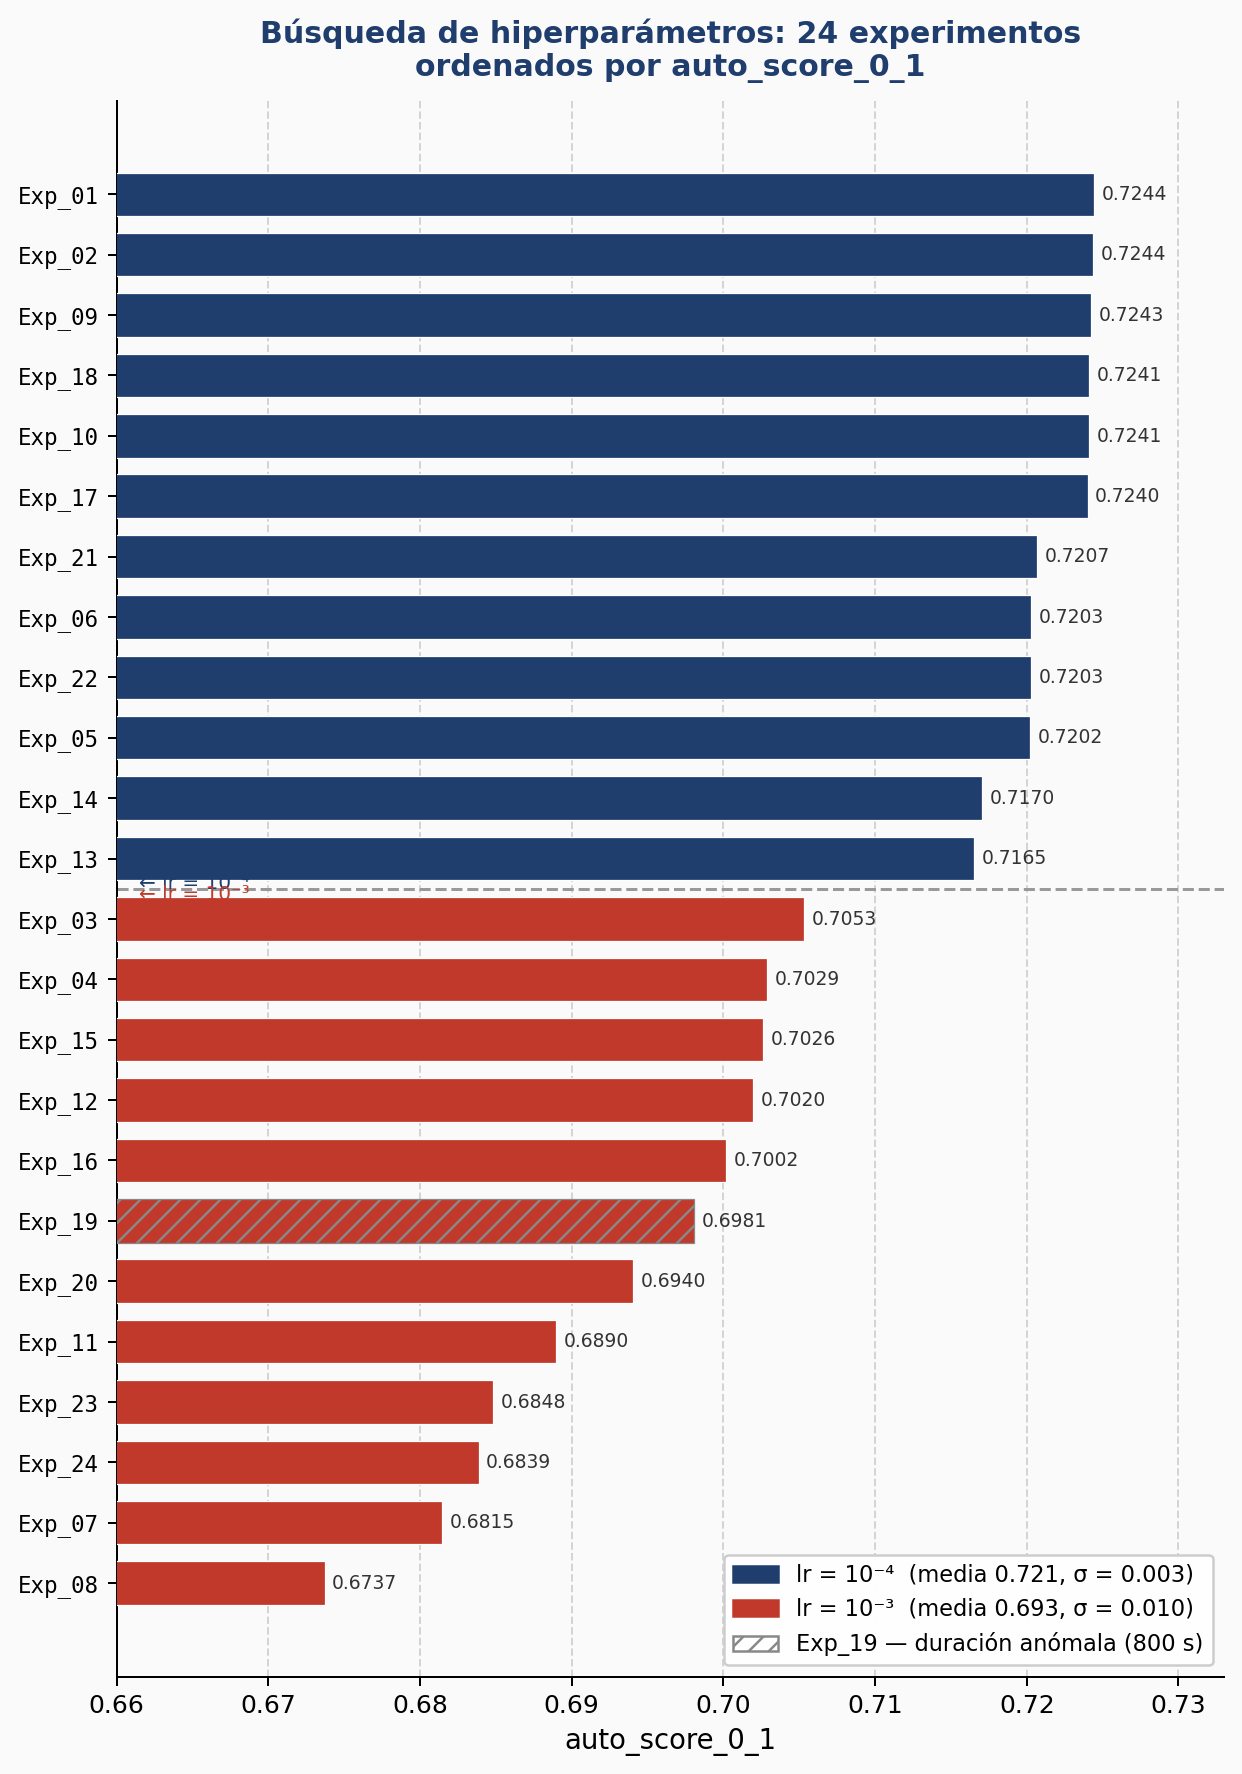
\includegraphics[width=0.72\textwidth]{figures/sweep_all_experiments.png}
    \caption{Los 24 experimentos de la b\'usqueda de hiperpar\'ametros ordenados por \texttt{auto\_score\_0\_1}. En azul, los experimentos con $\text{lr}=10^{-4}$; en rojo, los de $\text{lr}=10^{-3}$. La l\'inea discontinua marca el punto de corte entre ambos grupos. El experimento~19 (rayado) presenta duraci\'on an\'omala. Los 12 experimentos con $\text{lr}=10^{-4}$ ocupan las 12 primeras posiciones sin excepci\'on.}
    \label{fig:sweep-all-exps}
\end{figure}

\begin{table}[htbp]
    \centering
    \caption{Sensibilidad de \texttt{auto\_score\_0\_1} a cada hiperpar\'ametro}
    \label{tab:stage1-sensitivity}
    \begin{tabular}{llccc}
        \toprule
        \textbf{Hiperpar\'ametro} & \textbf{Valor} & \textbf{Media} & \textbf{Desv.\ t\'ip.} & \textbf{Efecto ($\Delta$)} \\
        \midrule
        Learning rate & $10^{-4}$ & 0.7217 & 0.0029 & \textbf{+0.029} \\
                      & $10^{-3}$ & 0.6932 & 0.0103 & \\
        \addlinespace
        Alpha         & 32        & 0.7114 & 0.0140 & +0.008 \\
                      & 128       & 0.7035 & 0.0181 & \\
        \addlinespace
        Rank          & 32        & 0.7066 & 0.0198 & $<0.001$ \\
                      & 64        & 0.7095 & 0.0128 & \\
                      & 128       & 0.7062 & 0.0178 & \\
        \addlinespace
        Dropout       & 0.05      & 0.7076 & 0.0163 & $<0.001$ \\
                      & 0.10      & 0.7072 & 0.0172 & \\
        \bottomrule
    \end{tabular}
\end{table}

Adem\'as, los experimentos con $\text{lr} = 10^{-3}$ presentan una variabilidad 3{,}5 veces mayor (desv.\ t\'ip.\ 0.0103 frente a 0.0029), lo que indica menor robustez de entrenamiento. Rank y dropout son pr\'acticamente irrelevantes en este contexto.

Las Figuras~\ref{fig:heatmap-rank-alpha} y~\ref{fig:sensitivity-lr} ilustran visualmente estos resultados.

\begin{figure}[htbp]
    \centering
    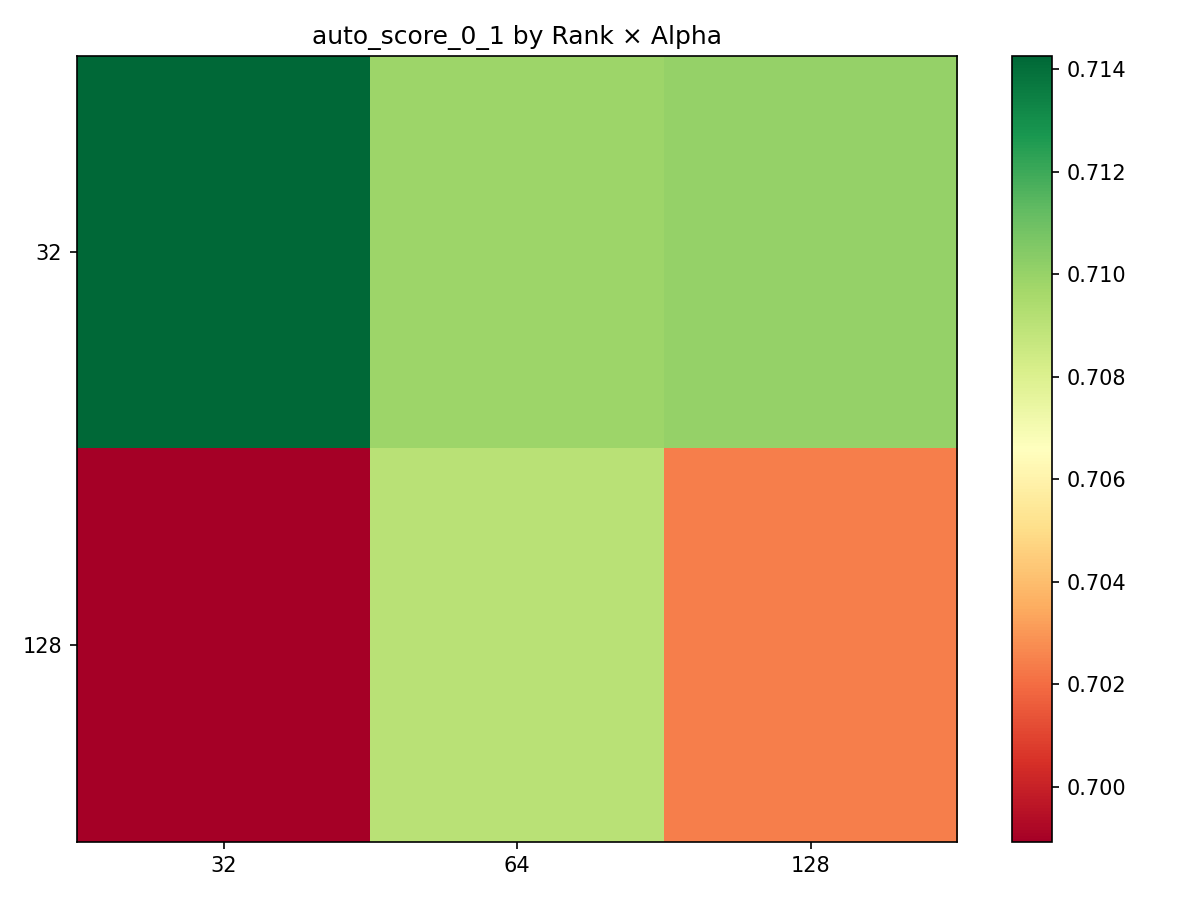
\includegraphics[width=0.72\textwidth]{figures/heatmap_rank_alpha.png}
    \caption{Mapa de calor de \texttt{auto\_score\_0\_1} en funci\'on de rank y alpha (media sobre lr y dropout). Los valores m\'as altos se concentran en alpha~=~32 independientemente del rank.}
    \label{fig:heatmap-rank-alpha}
\end{figure}

\begin{figure}[htbp]
    \centering
    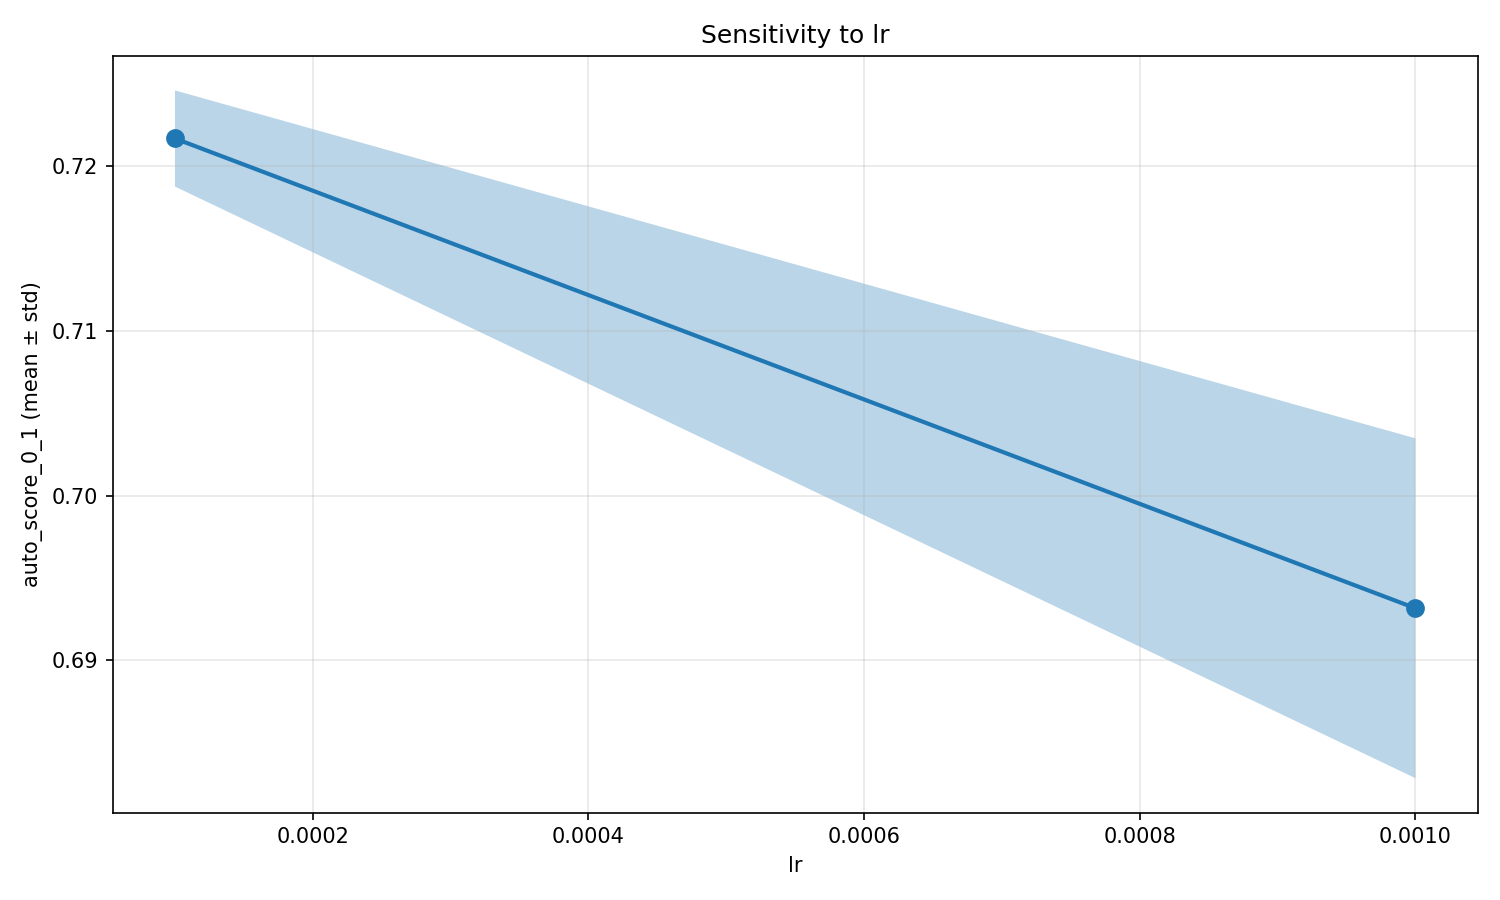
\includegraphics[width=0.72\textwidth]{figures/sensitivity_lr.png}
    \caption{Sensibilidad de \texttt{auto\_score\_0\_1} a la tasa de aprendizaje. La diferencia entre $10^{-4}$ y $10^{-3}$ es la mayor observada entre todos los hiperpar\'ametros explorados.}
    \label{fig:sensitivity-lr}
\end{figure}

\begin{figure}[htbp]
    \centering
    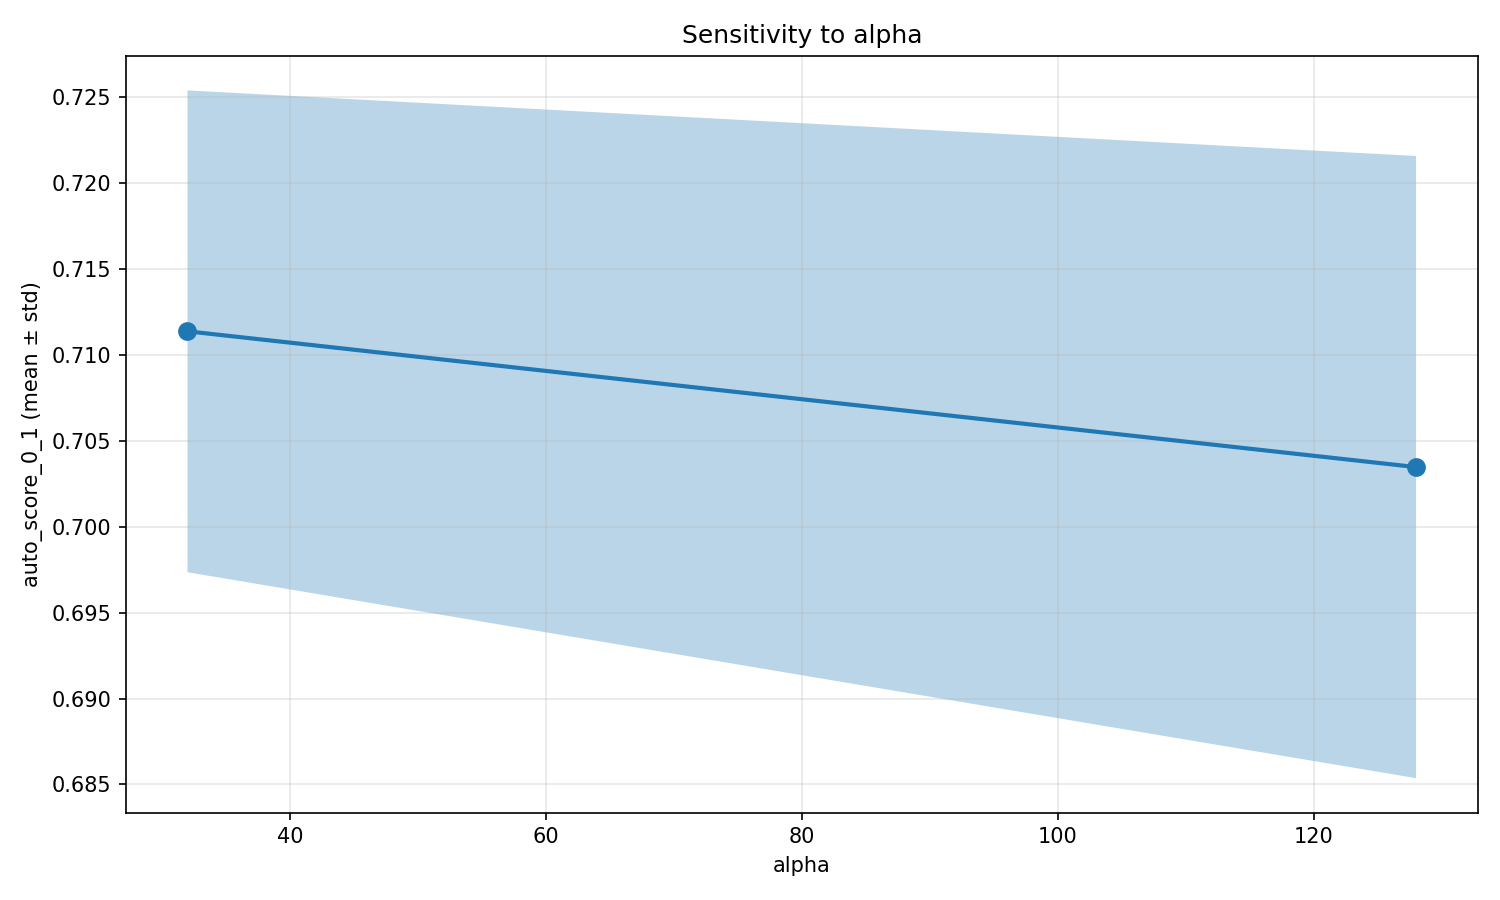
\includegraphics[width=0.72\textwidth]{figures/sensitivity_alpha.png}
    \caption{Sensibilidad de \texttt{auto\_score\_0\_1} al par\'ametro alpha. Alpha~=~32 supera consistentemente a alpha~=~128, especialmente en combinaci\'on con $\text{lr} = 10^{-4}$.}
    \label{fig:sensitivity-alpha}
\end{figure}

Se detect\'o una anomal\'ia en el experimento~19 (rank~=~128, alpha~=~32, $\text{lr} = 10^{-3}$, dropout~=~0.05): su duraci\'on de entrenamiento fue 800\,s frente a los ${\sim}$5400\,s del resto, lo que sugiere una interrupci\'on y reinicio parcial. El experimento alcanz\'o epoch~140 y su score (0.705) es coherente con el grupo $\text{lr} = 10^{-3}$; se mantiene en el an\'alisis como dato v\'alido con esta advertencia.

\section{Evaluaci\'on manual de la b\'usqueda de hiperpar\'ametros}
\label{s:stage1-manual}

Se evalu\'o auditivamente un subconjunto de checkpoints de los cinco experimentos con mejor ranking autom\'atico de la b\'usqueda, cubriendo dos epochs por experimento. La Tabla~\ref{tab:stage1-manual} recoge los promedios obtenidos.

\begin{table}[htbp]
    \centering
    \caption{Resultados de la evaluaci\'on manual de la b\'usqueda de hiperpar\'ametros (escala 0--20, 4 criterios)}
    \label{tab:stage1-manual}
    \small
    \begin{tabular}{lp{4.5cm}cccc}
        \toprule
        \textbf{Exp.} & \textbf{Config.} & \textbf{Epoch} & \textbf{Score} & \textbf{J\'onico} & \textbf{E\'olico} \\
        \midrule
        Exp\_01 & r32, $\alpha$32, lr$=10^{-4}$, do=0.05 & 80  & 8.48 & 7.63  & 12.63 \\
        Exp\_02 & r32, $\alpha$32, lr$=10^{-4}$, do=0.10 & 80  & 8.48 & 8.25  & 12.63 \\
        Exp\_09 & r64, $\alpha$32, lr$=10^{-4}$, do=0.05 & 60  & 8.66 & 7.13  & 13.00 \\
        Exp\_10 & r64, $\alpha$32, lr$=10^{-4}$, do=0.10 & 60  & 8.70 & 8.00  & 11.63 \\
        \textbf{Exp\_18} & \textbf{r128, $\alpha$32, lr$=10^{-4}$, do=0.10} & \textbf{120} & \textbf{9.89} & \textbf{12.13} & \textbf{12.25} \\
        \bottomrule
    \end{tabular}
\end{table}

De estos resultados se extraen dos hallazgos metodol\'ogicos relevantes.

\textbf{El epoch \'optimo no es el checkpoint final.} El protocolo de b\'usqueda evalu\'o autom\'aticamente epoch~140 para todos los experimentos. Sin embargo, Exp\_18 alcanza su mejor resultado en epoch~120 (9.89/20), y Exp\_09/10 pican en epoch~60 y caen en epoch~80. El uso sistem\'atico del checkpoint final infravalora configuraciones que convergen antes, lo que constituye una limitaci\'on del protocolo de evaluaci\'on autom\'atica empleado.

\textbf{El ranking autom\'atico no predice el mejor resultado perceptivo.} Exp\_01 obtiene el mayor \texttt{auto\_score\_0\_1} de toda la b\'usqueda (0.7244), pero solo 8.48/20 en evaluaci\'on manual. Exp\_18, cuarto en el ranking autom\'atico (0.7241, diferencia de apenas 0.0003), es el mejor perceptivamente con 9.89/20. Una diferencia de 0.0003 en la m\'etrica autom\'atica oculta 1.4 puntos de distancia en calidad auditiva real. Este resultado refuerza la necesidad del enfoque de evaluaci\'on dual: la m\'etrica autom\'atica es \'util para cribar el espacio de configuraciones, pero no puede sustituir a la escucha informada para determinar el mejor checkpoint.

La Figura~\ref{fig:auto-vs-manual} visualiza esta inversi\'on comparando la posici\'on de cada experimento en ambos rankings: Exp\_01 ocupa el primer puesto en el ranking autom\'atico pero el \'ultimo en el manual, mientras que Exp\_18 hace el camino inverso.

\begin{figure}[htbp]
    \centering
    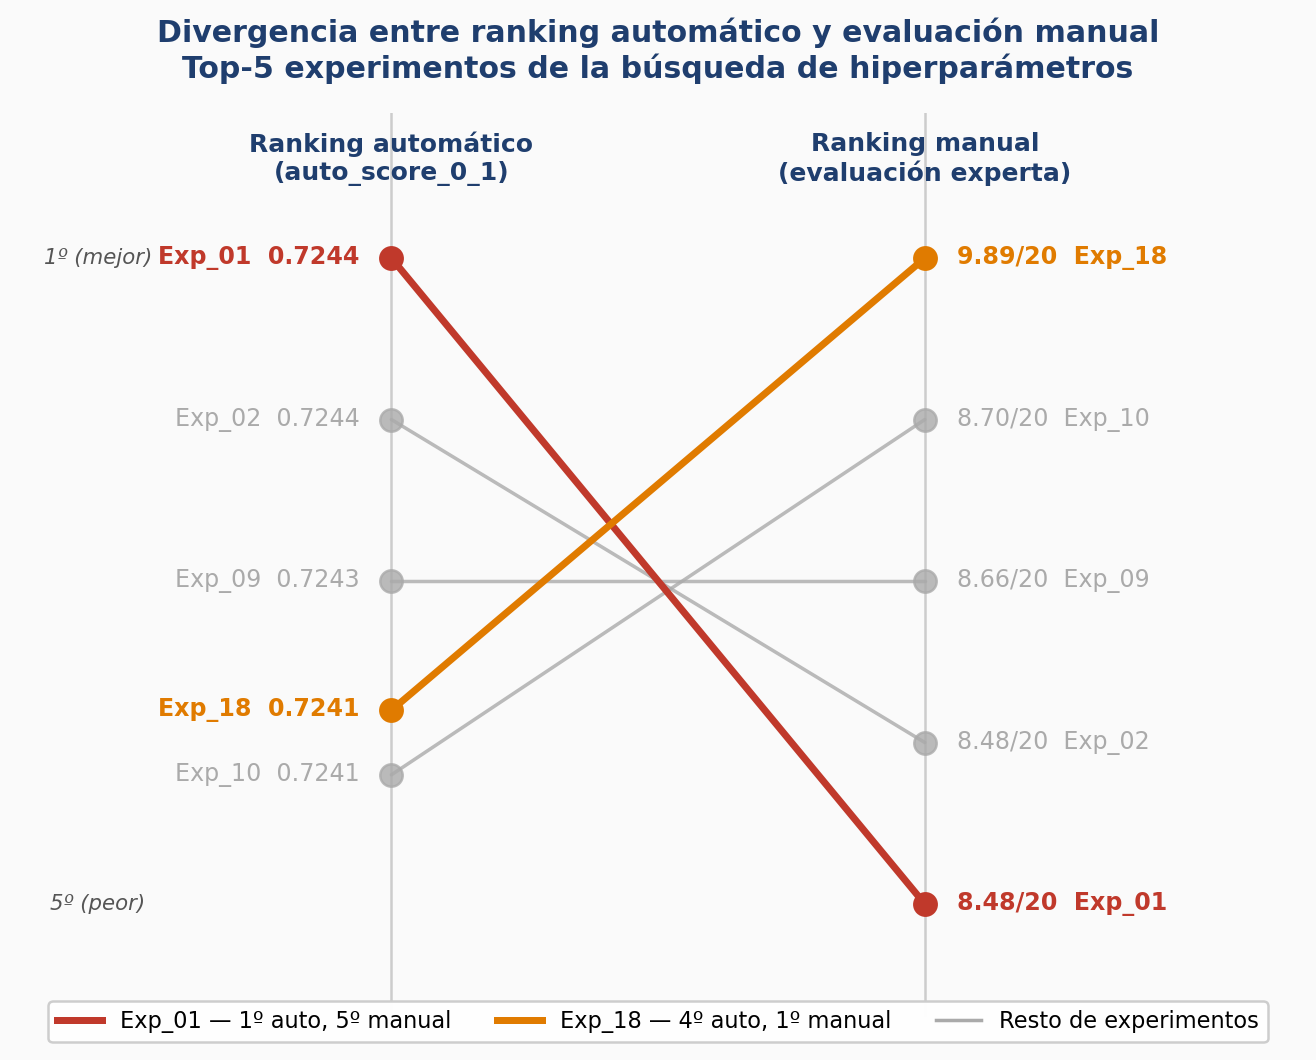
\includegraphics[width=0.85\textwidth]{figures/auto_vs_manual_top5.png}
    \caption{Posici\'on de los cinco experimentos mejor puntuados autom\'aticamente en el ranking autom\'atico (azul oscuro) y en el ranking de evaluaci\'on manual (azul claro). La barra m\'as corta indica mejor posici\'on (1 = mejor). Exp\_01 lidera el ranking autom\'atico pero queda \'ultimo en el manual; Exp\_18 ocupa la cuarta posici\'on autom\'atica pero la primera en escucha informada. Se incluyen los valores reales de \texttt{auto\_score\_0\_1} y la puntuaci\'on manual para referencia.}
    \label{fig:auto-vs-manual}
\end{figure}

Durante la escucha se observ\'o adem\'as un patr\'on de confusi\'on espec\'ifico de las configuraciones de la b\'usqueda que no aparec\'ia en run\_D: varios audios pedidos como e\'olico (menor natural) inclu\'ian de forma prominente la 2\textordfeminine\ disminuida, que es la nota caracter\'istica del frigio. Es decir, el modelo confunde un modo menor con otro modo menor distinto, en lugar de simplemente caer al mayor como en run\_D. Esta confusi\'on entre modos menores cercanos sugiere que la se\~nal de condicionamiento modal en estas configuraciones es menos n\'itida (probablemente por la combinaci\'on de una tasa de aprendizaje m\'as alta, $10^{-4}$ frente a $5\cdot10^{-5}$ de run\_D, y un n\'umero distinto de \'epocas evaluadas).

\section{Experimento de confirmaci\'on}
\label{s:experimento-confirmacion}
\label{s:confirm-exp}

A partir de los resultados de la b\'usqueda sistem\'atica de hiperpar\'ametros, que identific\'o $\text{lr} = 10^{-4}$ y $\alpha = 32$ como configuraci\'on dominante, se realiz\'o un experimento de confirmaci\'on con esa configuraci\'on \'optima ($r=32$, $\alpha=32$, $\text{lr}=10^{-4}$, dropout~=~0.05) para verificar si los resultados autom\'aticos se traducen en mejora perceptiva real frente al checkpoint de referencia run\_D.

La evaluaci\'on manual del experimento de confirmaci\'on se realiz\'o con los mismos cuatro criterios que el resto del estudio (centro tonal, color modal, no modulaci\'on y coherencia, escala 0--20). La Tabla~\ref{tab:confirm-comparativa} recoge la comparativa directa por modo frente a run\_D.

\begin{table}[htbp]
    \centering
    \caption{Comparativa directa entre run\_D y el experimento de confirmaci\'on (epoch~140, escala 0--20)}
    \label{tab:confirm-comparativa}
    \begin{tabular}{lcccc}
        \toprule
        \textbf{Modo} & \textbf{run\_D (/20)} & \textbf{run\_D \%} & \textbf{Confirmaci\'on (/20)} & \textbf{Confirm. \%} \\
        \midrule
        J\'onico              & 17.75 & 89\,\% & 16.25 & 81\,\% \\
        \textbf{D\'orico}     & 11.75 & 59\,\% & 14.13 & \textbf{71\,\%} \\
        Frigio                & 11.00 & 55\,\% &  9.38 & 47\,\% \\
        Lidio                 & 15.50 & 78\,\% & 11.00 & 55\,\% \\
        Mixolidio             & 12.00 & 60\,\% & 10.50 & 53\,\% \\
        E\'olico              & 11.38 & 57\,\% & 10.00 & 50\,\% \\
        Locrio                &  7.50 & 38\,\% &  6.63 & 33\,\% \\
        \midrule
        \textbf{Global} & \textbf{12.41/20} & \textbf{62\,\%} & \textbf{11.14/20} & \textbf{56\,\%} \\
        \bottomrule
    \end{tabular}
\end{table}

El experimento de confirmaci\'on no mejora el resultado global de run\_D (56\,\% frente a 62\,\%), pero logra el objetivo espec\'ifico para el que fue dise\~nado: reducir el sesgo hacia sonoridades mayores en los modos menores. El hallazgo m\'as relevante es la mejora en modo d\'orico (+12\,pp): run\_D alcanzaba un 59\,\% en ese modo con tendencia sistem\'atica a generar D~mayor en lugar de D~menor, mientras que el experimento de confirmaci\'on alcanza un 71\,\%, con ejemplos donde el car\'acter d\'orico es claramente perceptible (6\textordfeminine\ mayor prominente, variaciones arm\'onicas caracter\'isticas del modo). \'Esta es la primera configuraci\'on del estudio que produce ejemplos d\'oricos reconocibles de forma consistente.

Esta mejora tiene un coste: la capacidad del adaptador se redistribuye hacia los modos menores, lo que reduce ligeramente el rendimiento en modos mayores ya bien dominados por el modelo base, especialmente en lidio ($-23$\,pp) y j\'onico ($-8$\,pp).

La Figura~\ref{fig:comparativa-runD-confirm} visualiza la comparativa completa por modo, ilustrando tanto el patr\'on general de retroceso de la configuraci\'on de confirmaci\'on como la excepci\'on notable en d\'orico.

\begin{figure}[htbp]
    \centering
    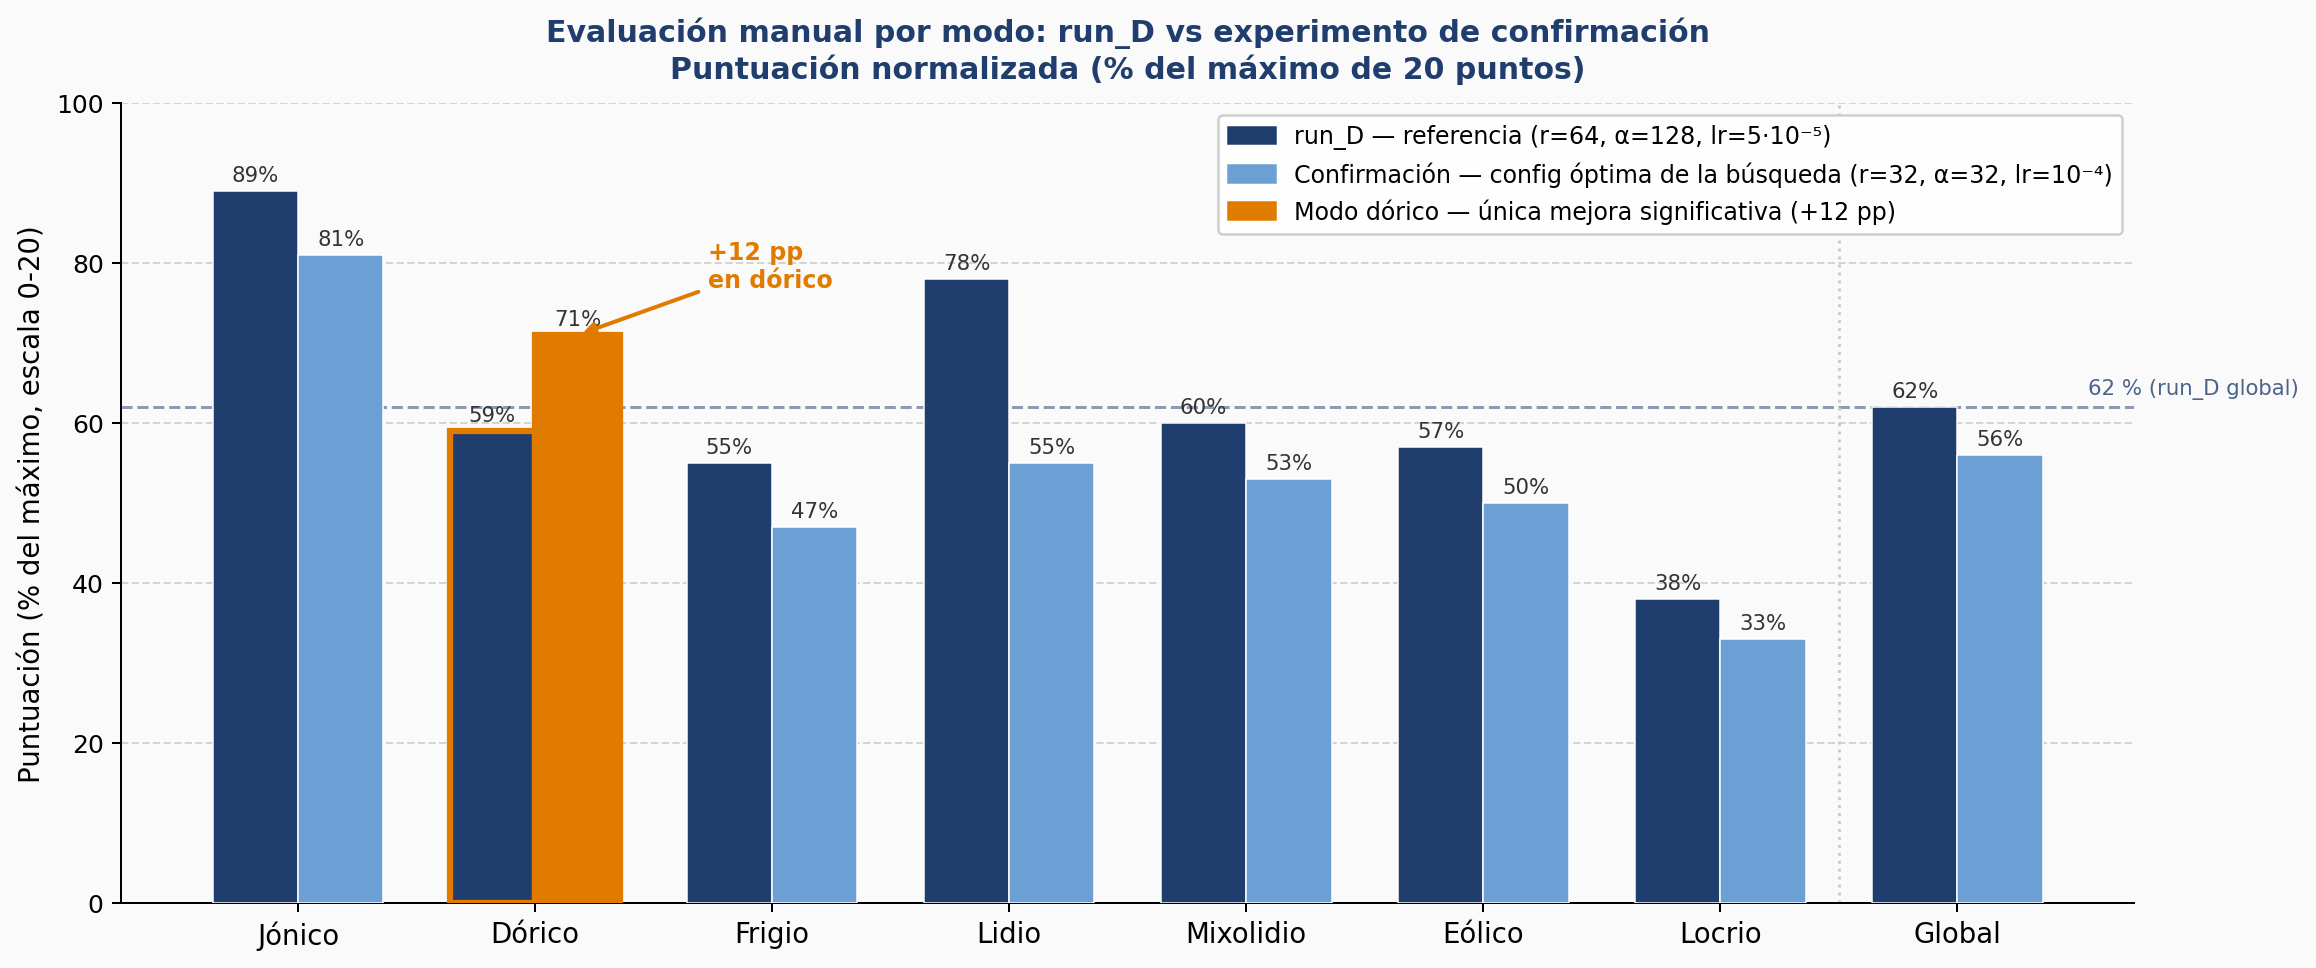
\includegraphics[width=\textwidth]{figures/comparativa_runD_confirm.png}
    \caption{Comparativa de la evaluaci\'on manual por modo entre run\_D y el experimento de confirmaci\'on. Las barras representan el porcentaje del m\'aximo de 20 puntos. La l\'inea discontinua marca el promedio global de run\_D (62\,\%). El modo d\'orico (naranja) es el \'unico con mejora significativa (+12\,pp); el resto retrocede entre 5 y 23 puntos porcentuales.}
    \label{fig:comparativa-runD-confirm}
\end{figure}

\section{An\'alisis cualitativo por modo}
\label{s:analisis-cualitativo-modos}

M\'as all\'a de los valores num\'ericos, la evaluaci\'on auditiva permiti\'o identificar patrones cualitativos consistentes en c\'omo el modelo trata cada modo. Este an\'alisis complementa la tabla de resultados con observaciones sobre el tipo de error m\'as frecuente, la nota caracter\'istica que el modelo tiende a ignorar y el nivel de consistencia perceptiva dentro de cada modo.

\textbf{J\'onico (89\,\% en run\_D).} Es el modo mejor controlado del estudio, lo que refleja el sesgo del modelo base hacia sonoridades mayores. La t\'onica se establece con claridad desde los primeros compases, las progresiones arm\'onicas son coherentes y la calidad t\'imbrica es alta. El riesgo principal es el opuesto: el modelo puede generar j\'onico cuando se le pide otro modo mayor (lidio o mixolidio), diluyendo la separabilidad entre ellos.

\textbf{D\'orico (59\,\% en run\_D; 71\,\% en confirmaci\'on).} Es el modo que experimenta la mejora m\'as significativa del estudio (+12\,pp). El problema central en run\_D es que el modelo genera D~menor natural en lugar de D~d\'orico: omite sistem\'aticamente la 6\textordfeminine\ mayor (Si$\natural$) y produce la 6\textordfeminine\ menor (Si$\flat$), que es la nota caracter\'istica del e\'olico. Con la configuraci\'on de confirmaci\'on aparecen por primera vez fragmentos donde el Si$\natural$ es claramente audible, con progresiones arm\'onicas que incluyen acordes de II~mayor o VI~mayor, rasgos arm\'onicos distintivos del d\'orico en jazz.

\textbf{Frigio (55\,\% en run\_D).} El modo frigio presenta el reto de la 2\textordfeminine\ disminuida sobre la t\'onica, que en el caso de E~frigio implica usar Fa$\natural$ sobre Mi. El modelo tiende a evitar este intervalo y genera la 2\textordfeminine\ mayor (Fa$\sharp$), aproximando la salida a E~menor natural. Cuando aparecen rasgos frigios, lo hacen de forma puntual ---en una frase o en la cadencia--- pero sin mantenerse durante toda la pieza. El estilo flamenco o \'arabe que caracteriza al frigio no emerge de forma consistente en ninguna configuraci\'on evaluada.

\textbf{Lidio (78\,\% en run\_D).} Junto al j\'onico, es el modo con mejor resultado en run\_D. La 4\textordfeminine\ aumentada (Si$\natural$ en F~lidio) aparece con frecuencia en las melodías, y el car\'acter et\'ereo o flotante del modo es perceptible. El retroceso en confirmaci\'on ($-23$\,pp) se interpreta como un efecto de la menor capacidad del adaptador ($r=32$ frente a $r=64$) para mantener la separabilidad en modos que requieren diferenciaci\'on espectral m\'as fina respecto al mayor natural.

\textbf{Mixolidio (60\,\% en run\_D).} El modo mixolidio se diferencia del j\'onico \'unicamente por la 7\textordfeminine\ menor. El modelo casi nunca introduce esa nota de forma prominente: las salidas etiquetadas como mixolidio suenan en su mayor\'ia a mayor natural, con la 7\textordfeminine\ apareciendo ocasionalmente en pasajes de relleno arm\'onico. El car\'acter bluesy o celta que define al mixolidio ---donde la 7\textordfeminine\ menor crea tensi\'on sobre el acorde de t\'onica--- rara vez emerge de forma convincente.

\textbf{E\'olico (57\,\% en run\_D).} El menor natural es el modo al que el modelo parece recurrir como \textit{default} cuando se le pide una sonoridad oscura. Las salidas son funcionalmente correctas como m\'usica en menor, pero carecen de diferenciaci\'on clara respecto al d\'orico o el frigio: la 6\textordfeminine\ puede ser mayor o menor seg\'un la frase, y la 7\textordfeminine\ no siempre es la mayor esperada. El modo e\'olico obtiene resultados aceptables precisamente porque es el modo menor m\'as neutro, no porque el modelo lo controle con precisi\'on.

\textbf{Locrio (38\,\% en run\_D).} Es el modo m\'as dif\'icil de controlar y el que peores resultados obtiene en todas las configuraciones evaluadas. El tr\'itono entre la t\'onica y la quinta disminuida genera una inestabilidad arm\'onica tan acusada que el modelo tiende a resolver de inmediato hacia otra tonalidad: las escuchas revelan que la m\'usica empieza en un contexto ambiguo pero termina estabiliz\'andose en B~mayor, E~mayor o incluso A~menor, sin mantener en ning\'un momento el centro tonal en Si. Este comportamiento es coherente con la pr\'actica habitual en m\'usica popular, donde locrio casi nunca se sostiene durante m\'as de unos pocos acordes. El experimento de confirmaci\'on obtiene 0.705 frente a 0.711 de run\_D, un nuevo caso donde \texttt{auto\_score\_0\_1} infravalora mejoras perceptivas en modos menores con car\'acter modal sutil. Esto refuerza la necesidad de evaluaci\'on dual.

\section{An\'alisis por modo del checkpoint de referencia run\_D}
\label{s:analisis-modos-ref}

Tomando como referencia la mejor configuraci\'on de la fase exploratoria (r64-a128-d0.05-lr5e-5, epoch~100, run\_D), la Tabla~\ref{tab:analisis-modos} recoge la media por modo sobre la escala de evaluaci\'on manual (0--20). Esta tabla establece la l\'inea de referencia que el experimento de confirmaci\'on (Secci\'on~\ref{s:confirm-exp}) toma como punto de partida para reducir el sesgo en modos menores.

\begin{table}[htbp]
    \centering
    \caption{Media por modo en el checkpoint de referencia run\_D ($r=64$, $\alpha=128$, $\text{lr}=5\cdot10^{-5}$, epoch~100)}
    \label{tab:analisis-modos}
    \begin{tabular}{lcl}
        \toprule
        \textbf{Modo} & \textbf{Media} & \textbf{Interpretaci\'on} \\
        \midrule
        J\'onico & 17.75 & Muy buen control y coherencia global \\
        Lidio & 15.50 & Buen control modal con ejemplos destacados \\
        Mixolidio & 12.00 & Control parcial, confusi\'on ocasional con sonoridad mayor natural \\
        D\'orico & 11.75 & Color modal parcial, tendencia a resolver en mayor \\
        Frigio & 11.00 & Rasgos parciales, inestabilidad en sonoridad menor \\
        E\'olico & 11.38 & Resultado funcional pero poco consistente en color modal \\
        Locrio & 7.50 & Modo menos robusto e inestable \\
        \bottomrule
    \end{tabular}
\end{table}

El patr\'on observado es coherente con las escuchas: el modelo responde mejor en modos con sonoridad m\'as estable y presenta m\'as dificultad en modos con mayor tensi\'on arm\'onica, especialmente en locrio y en parte de los modos menores.

\section{Patr\'on de confusi\'on mayor/menor}
\label{s:confusion-mayor-menor}

El an\'alisis cualitativo de las escuchas revela un sesgo sistem\'atico y recurrente: el modelo tiende a generar los modos menores (d\'orico, frigio, e\'olico) en su relativo o paralelo mayor. Este comportamiento aparece de forma consistente en todos los runs evaluados y no se corrige con mayor n\'umero de epochs dentro del rango explorado.

La Tabla~\ref{tab:patron-confusion} documenta las confusiones m\'as frecuentes observadas durante la evaluaci\'on manual.

\begin{table}[htbp]
    \centering
    \caption{Confusiones recurrentes entre modo objetivo y modo generado}
    \label{tab:patron-confusion}
    \begin{tabular}{llp{5.5cm}}
        \toprule
        \textbf{Modo objetivo} & \textbf{Generado} & \textbf{Observaci\'on t\'ipica} \\
        \midrule
        D\'orico (D menor)    & D mayor           & ``No aprende que el d\'orico es un modo menor'' \\
        Frigio (E menor)      & E mayor           & ``No capta el menor; suena la 7\textordfeminine\ mayor'' \\
        Mixolidio (G mix.)    & G mayor natural   & ``No mete la 7\textordfeminine\ menor en ning\'un momento'' \\
        E\'olico (A menor)    & A menor (parcial) & ``Falta la 6\textordfeminine\ menor caracter\'istica'' \\
        Locrio (B loc.)       & B/E mayor         & ``No consolida la ra\'iz en B; muy inestable'' \\
        \bottomrule
    \end{tabular}
\end{table}

Este patr\'on sugiere que el modelo base de ACE-Step tiene un sesgo inherente hacia sonoridades mayores y resoluciones ton\'ales est\'ables, que la adaptaci\'on LoRA no logra revertir completamente con el dataset y configuraci\'on actuales. La implicaci\'on pr\'actica es que mejorar el control en modos menores requerir\'ia bien aumentar la proporci\'on de ejemplos de entrenamiento en esos modos, bien utilizar una se\~nal de condicionamiento m\'as expl\'icita que distinga activamente entre modo mayor y menor.

\section{Ablaci\'on de variantes de prompt}
\label{s:ablacion-prompts}

Sobre el mismo checkpoint base (epoch~100, run\_D), se evalu\'o el efecto de tres variantes de prompt para aislar la contribuci\'on del condicionamiento textual:

\begin{itemize}
    \item \textbf{Bloque B (detallado):} descripci\'on modal completa con t\'onica, car\'acter arm\'onico y contexto de jazz-fusi\'on.
    \item \textbf{Bloque modo+instrumento:} nombre del modo con instrumentaci\'on, sin t\'onica expl\'icita.
    \item \textbf{Bloque modo solo:} \'unicamente el nombre del modo.
\end{itemize}

La Tabla~\ref{tab:ablacion-prompts} recoge los promedios globales y el valor por modo en d\'orico, donde la diferencia es m\'as pronunciada.

\begin{table}[htbp]
    \centering
    \caption{Comparativa de variantes de prompt sobre el mismo checkpoint (epoch~100)}
    \label{tab:ablacion-prompts}
    \begin{tabular}{lccc}
        \toprule
        \textbf{Variante de prompt} & \textbf{Promedio global} & \textbf{D\'orico} & \textbf{J\'onico} \\
        \midrule
        B (detallado)         & 10.48 & 9.00  & 17.38 \\
        Modo + instrumento    & 10.52 & 7.75  & 16.50 \\
        \textbf{Modo solo}    & \textbf{10.79} & \textbf{9.75} & 16.25 \\
        \bottomrule
    \end{tabular}
\end{table}

El prompt m\'as minimalista (\textit{modo solo}) supera a los m\'as detallados en promedio global y especialmente en d\'orico. Esto sugiere que el condicionamiento textual excesivo puede interferir con la se\~nal modal aprendida por el adaptador, posiblemente porque el modelo base ya resuelve bien ciertos aspectos musicales a partir de pocas palabras clave. Este resultado es relevante para RQ3: la evaluaci\'on reproducible del control modal no debe asumir que m\'as contexto textual implica mejor resultado.

\section{Comparativa global de configuraciones}
\label{s:comparativa-global}

Una vez analizados individualmente la fase exploratoria, la b\'usqueda sistem\'atica y el experimento de confirmaci\'on, la Tabla~\ref{tab:comparativa-runs} sintetiza el comportamiento medio de las configuraciones m\'as representativas evaluadas a lo largo del estudio. Los valores corresponden a la media global de la r\'ubrica manual para los checkpoints m\'as representativos de cada configuraci\'on.

\begin{table}[htbp]
    \centering
    \caption{Comparativa resumida de configuraciones LoRA evaluadas}
    \label{tab:comparativa-runs}
    \small
    \begin{tabular}{p{3.8cm}lcp{4.8cm}}
        \toprule
        \textbf{Configuraci\'on} & \textbf{Checkpoint} & \textbf{Media} & \textbf{Observaci\'on} \\
        \midrule
        r128-a256-d0.05 & epoch 20  & 10.79 & Calidad aceptable inicial, inestable en modos \\
        r128-a256-d0.05 & epoch 100 & 5.82  & Degradaci\'on fuerte (sobreentrenamiento) \\
        r64-a128-d0     & epoch 80  & 9.57  & Resultado medio, control modal parcial \\
        r64-a128-d0     & epoch 180 & 9.29  & Estancamiento respecto a checkpoints previos \\
        r64-a128-d0.05  & epoch 160 & 5.09  & Configuraci\'on descartada por baja calidad \\
        r64-a128-d0.05-lr5e-5 & epoch 100 & 12.41 & Configuraci\'on de referencia (run\_D) \\
        r64-a128-d0.05-lr5e-5 & epoch 140 & 9.96  & Ca\'ida respecto al mejor checkpoint \\
        r64-a128-d0.05-lr5e-5 & epoch 160 & 10.34 & Recuperaci\'on parcial, inferior a epoch 100 \\
        \midrule
        confirm-r32-a32-lr1e-4$^{*}$ & epoch 140 & 11.14 & Mejor resultado en modos menores; ver Secci\'on~\ref{s:confirm-exp} \\
        \bottomrule
        \multicolumn{4}{p{13cm}}{$^{*}$ Escala 0--20 (4 criterios). Equivale a 55.7\,\% del m\'aximo frente al 62.1\,\% de run\_D (ambos sobre~20). Mejora en d\'orico: +12\,pp.}
    \end{tabular}
\end{table}

Esta comparativa sugiere dos conclusiones relevantes: (i) aumentar capacidad ($r$ y $\alpha$ altos) no garantiza mejor control modal sostenido y puede degradar resultados; (ii) la configuraci\'on m\'as equilibrada de la fase exploratoria es run\_D, pero el experimento de confirmaci\'on derivado de la b\'usqueda sistem\'atica reduce de forma espec\'ifica el sesgo en modos menores ---especialmente en d\'orico--- a costa de un ligero retroceso global.

\section{Hallazgos principales}

El resultado m\'as relevante es que el condicionamiento modal mediante LoRA es viable sobre ACE-Step 1.5 sin reentrenar el modelo completo. No obstante, persiste una limitaci\'on en la consolidaci\'on de ciertos modos menores, que en algunos casos tienden a confundirse con sonoridades m\'as estables de tipo mayor.

Este comportamiento sugiere que el principal reto ya no es la calidad t\'imbrica, sino la separaci\'on arm\'onica fina entre modos cercanos. Por tanto, los siguientes ciclos experimentales deben priorizarse en esa direcci\'on y no en aumentar complejidad superficial de prompts.

Como consecuencia pr\'actica, los hallazgos de la b\'usqueda de hiperpar\'ametros orientaron directamente un experimento de confirmaci\'on con $\text{lr} = 10^{-4}$, $\alpha = 32$ y $r = 32$. Este experimento no supera a run\_D en el resultado global (56\,\% frente a 62\,\%), pero valida su objetivo espec\'ifico: reducir el sesgo en modo d\'orico (+12 puntos porcentuales, de 59\,\% a 71\,\%), siendo la primera configuraci\'on del estudio que produce ejemplos d\'oricos reconocibles de forma consistente. El ciclo experimental queda as\'i cerrado: b\'usqueda sistem\'atica, identificaci\'on de configuraci\'on \'optima para el modo problem\'atico y validaci\'on emp\'irica focalizada.

\section{Respuesta a las preguntas de investigaci\'on}

Con la evidencia disponible en esta fase del proyecto, puede responderse de forma provisional a las preguntas planteadas en la introducci\'on:

\begin{itemize}
    \item \textbf{RQ1:} S\'i, LoRA permite mejorar control modal manteniendo calidad global razonable, aunque el efecto no es homog\'eneo en todos los modos.
    \item \textbf{RQ2:} La b\'usqueda sistem\'atica identifica $\text{lr} = 10^{-4}$ y $\alpha = 32$ como configuraci\'on dominante. Un experimento de confirmaci\'on posterior valida el objetivo espec\'ifico de esa configuraci\'on: reducir el sesgo en modo d\'orico (+12\,pp, de 59\,\% a 71\,\%), siendo el primer resultado del estudio con ejemplos d\'oricos reconocibles de forma consistente, aunque el promedio global desciende ligeramente (56\,\% frente a 62\,\% de run\_D). El ciclo completo ---b\'usqueda $\to$ identificaci\'on $\to$ confirmaci\'on--- demuestra la utilidad pr\'actica de la metodolog\'ia propuesta.
    \item \textbf{RQ3:} Una evaluaci\'on reproducible para modalidad requiere enfoque dual; las m\'etricas autom\'aticas son \'utiles para cribar, pero insuficientes sin validaci\'on auditiva estructurada.
\end{itemize}

\section{Validez y limitaciones}

Entre las principales limitaciones del estudio destacan el tama\~no reducido del dataset y su desbalance entre clases. Adem\'as, la evaluaci\'on humana, aunque estructurada, mantiene una componente subjetiva: las puntuaciones de la r\'ubrica fueron asignadas por un \'unico evaluador (el autor de este trabajo), por lo que no se dispone de medida de acuerdo inter-evaluadores. Esto debe tenerse en cuenta al interpretar diferencias peque\~nas entre configuraciones.

Otra limitaci\'on de car\'acter estad\'istico es la b\'usqueda sistem\'atica de hiperpar\'ametros: cada configuraci\'on se evalu\'o con $n=2$ semillas por modo (1111 y 2222), un n\'umero suficiente para detectar efectos grandes (como el de la tasa de aprendizaje, $\Delta=0.029$) pero insuficiente para distinguir con confianza diferencias inferiores a $\sim$0.005 en \texttt{auto\_score\_0\_1}. Las primeras posiciones del ranking de la Tabla~\ref{tab:stage1-top10}, separadas por d\'ecimas de mil\'esima, deben interpretarse como un grupo de configuraciones equivalentes m\'as que como un orden estricto.

Como punto fuerte, el protocolo seguido es reproducible y permite tomar decisiones experimentales con criterios expl\'icitos.

Otra limitaci\'on relevante es que la evaluaci\'on auditiva exige mucho tiempo cuando se comparan muchos checkpoints y semillas. Para mitigarlo, el flujo adoptado combina filtrado autom\'atico determinista y evaluaci\'on manual focalizada en candidatos, lo que mejora la eficiencia sin perder control metodol\'ogico.

Respecto al dataset, los 102 clips se obtuvieron a partir de fragmentos cortos (20--50\,s) de obras musicales existentes, seleccionados manualmente con fines exclusivamente acad\'emicos y de investigaci\'on. El material no se redistribuye con el repositorio: \'unicamente se publican los tensores latentes precalculados por el VAE de ACE-Step, que constituyen una representaci\'on derivada no invertible a audio original. Esta decisi\'on es coherente con el uso justo en contexto educativo y con la pr\'actica habitual en investigaci\'on con modelos generativos sobre material protegido. No obstante, el dataset no es redistribuible en su forma original y constituye una limitaci\'on de reproducibilidad externa que se asume expl\'icitamente.

\chapter{Conclusiones y trabajo futuro}
\label{ch:conclusiones}

\section{Conclusiones}

Se concluye que:

\begin{enumerate}
    \item La adaptaci\'on LoRA sobre ACE-Step 1.5 permite introducir control modal sin reentrenamiento completo, con coste computacional razonable para iteraci\'on acad\'emica.
    \item La b\'usqueda sistem\'atica de hiperpar\'ametros (24 experimentos) identifica la tasa de aprendizaje como el hiperpar\'ametro m\'as cr\'itico ($\Delta = 0.029$ en \texttt{auto\_score\_0\_1}), con $\text{lr} = 10^{-4}$ y $\alpha = 32$ como configuraci\'on dominante. Un experimento de confirmaci\'on posterior valida esta elecci\'on: aunque el resultado global desciende ligeramente (56\,\% frente a 62\,\% de run\_D), se logra por primera vez control d\'orico reconocible de forma consistente (+12 puntos porcentuales en ese modo, de 59\,\% a 71\,\%).
    \item El reto t\'ecnico principal no es la calidad sonora ---que se mantiene en niveles aceptables en todas las configuraciones--- sino la separaci\'on robusta entre modos cercanos, en particular entre modos menores y sus relativos mayores. El experimento de confirmaci\'on aten\'ua parcialmente este sesgo, aunque no lo elimina.
\end{enumerate}

En conjunto, los objetivos del proyecto se consideran alcanzados: se ha establecido una metodolog\'ia experimental completa y reproducible, se han identificado las configuraciones LoRA m\'as prometedoras mediante b\'usqueda sistem\'atica, y se ha validado emp\'iricamente que la configuraci\'on \'optima reduce de forma medible el sesgo en modos menores, con avances especialmente significativos en el modo d\'orico (+12\,pp en evaluaci\'on perceptiva).

Como cierre, la principal aportaci\'on del trabajo no es solo una configuraci\'on concreta, sino un procedimiento experimental replicable para estudiar control arm\'onico en modelos generativos musicales con recursos acotados.

\section{Trabajo futuro}

Como l\'ineas de continuaci\'on se plantean:

\begin{itemize}
    \item Extender el experimento de confirmaci\'on a m\'as configuraciones de rank y a mayor n\'umero de epochs, evaluando checkpoints intermedios para identificar el punto \'optimo de convergencia de forma m\'as precisa.
    \item Mejorar el balance del dataset en modos menos representados para reducir sesgos de aprendizaje modal.
    \item Refinar la estrategia de etiquetado modal conservador para aumentar separabilidad entre modos sin forzar caracter\'isticas ajenas al contenido real de los clips.
    \item Incorporar m\'etricas autom\'aticas complementarias para reducir carga de evaluaci\'on manual y facilitar escalado experimental.
    \item Validar resultados en m\'as semillas y escenarios de inferencia para estimar robustez fuera del conjunto de pruebas principal.
    \item Extender la evaluaci\'on manual de la b\'usqueda de hiperpar\'ametros al resto de experimentos no evaluados, para completar la validaci\'on auditiva del ranking autom\'atico m\'as all\'a de los cinco experimentos cubiertos (Exp\_01, Exp\_02, Exp\_09, Exp\_10, Exp\_18).
    \item Dise\~nar estrategias espec\'ificas para modos menores (d\'orico, frigio) que contrarresten el sesgo hacia sonoridades mayores identificado en la evaluaci\'on manual, como sobrerepresentaci\'on de esos modos en el dataset o refuerzo expl\'icito de la nota caracter\'istica en los captions.
\end{itemize}

\appendix

\chapter{Resultados completos de la b\'usqueda de hiperpar\'ametros}
\label{ap:stage1-completo}

La Tabla~\ref{tab:stage1-completo} recoge los 24 experimentos de la b\'usqueda sistem\'atica de hiperpar\'ametros, ordenados por identificador. El experimento~19 presenta una duraci\'on de entrenamiento an\'omala (800\,s frente a ${\sim}$5400\,s del resto); v\'ease la discusi\'on en el cap\'itulo de resultados.

\begin{table}[htbp]
    \centering
    \caption{Resultados completos de la b\'usqueda de hiperpar\'ametros (24 experimentos, epoch~140)}
    \label{tab:stage1-completo}
    \resizebox{\textwidth}{!}{%
    \begin{tabular}{cccccccc}
        \toprule
        \textbf{Exp.} & \textbf{Rank} & \textbf{Alpha} & \textbf{LR} & \textbf{do} & \textbf{Score} & \textbf{Acc.\ modal} & \textbf{Est.\ tonal} \\
        \midrule
        1  & 32  & 32  & $10^{-4}$ & 0.05 & 0.7244 & 0.7416 & 0.8932 \\
        2  & 32  & 32  & $10^{-4}$ & 0.10 & 0.7244 & 0.7416 & 0.8932 \\
        3  & 32  & 32  & $10^{-3}$ & 0.05 & 0.7053 & 0.7148 & 0.8872 \\
        4  & 32  & 32  & $10^{-3}$ & 0.10 & 0.7029 & 0.7134 & 0.8807 \\
        5  & 32  & 128 & $10^{-4}$ & 0.05 & 0.7202 & 0.7344 & 0.8936 \\
        6  & 32  & 128 & $10^{-4}$ & 0.10 & 0.7203 & 0.7346 & 0.8940 \\
        7  & 32  & 128 & $10^{-3}$ & 0.05 & 0.6815 & 0.6777 & 0.8874 \\
        8  & 32  & 128 & $10^{-3}$ & 0.10 & 0.6737 & 0.6754 & 0.8639 \\
        9  & 64  & 32  & $10^{-4}$ & 0.05 & 0.7243 & 0.7418 & 0.8896 \\
        10 & 64  & 32  & $10^{-4}$ & 0.10 & 0.7241 & 0.7417 & 0.8891 \\
        11 & 64  & 32  & $10^{-3}$ & 0.05 & 0.6890 & 0.6944 & 0.8789 \\
        12 & 64  & 32  & $10^{-3}$ & 0.10 & 0.7020 & 0.7106 & 0.8869 \\
        13 & 64  & 128 & $10^{-4}$ & 0.05 & 0.7165 & 0.7308 & 0.8855 \\
        14 & 64  & 128 & $10^{-4}$ & 0.10 & 0.7170 & 0.7313 & 0.8859 \\
        15 & 64  & 128 & $10^{-3}$ & 0.05 & 0.7026 & 0.7108 & 0.8928 \\
        16 & 64  & 128 & $10^{-3}$ & 0.10 & 0.7002 & 0.7111 & 0.8813 \\
        17 & 128 & 32  & $10^{-4}$ & 0.05 & 0.7240 & 0.7428 & 0.8889 \\
        18 & 128 & 32  & $10^{-4}$ & 0.10 & 0.7241 & 0.7429 & 0.8873 \\
        19$^{*}$ & 128 & 32 & $10^{-3}$ & 0.05 & 0.6981 & 0.7058 & 0.8828 \\
        20 & 128 & 32  & $10^{-3}$ & 0.10 & 0.6940 & 0.6994 & 0.8844 \\
        21 & 128 & 128 & $10^{-4}$ & 0.05 & 0.7207 & 0.7353 & 0.8902 \\
        22 & 128 & 128 & $10^{-4}$ & 0.10 & 0.7203 & 0.7350 & 0.8904 \\
        23 & 128 & 128 & $10^{-3}$ & 0.05 & 0.6848 & 0.6895 & 0.8716 \\
        24 & 128 & 128 & $10^{-3}$ & 0.10 & 0.6839 & 0.6894 & 0.8623 \\
        \bottomrule
        \multicolumn{8}{l}{$^{*}$ Duraci\'on an\'omala: 800\,s frente a ${\sim}$5400\,s del resto.}
    \end{tabular}}% cierre resizebox
\end{table}

\chapter{Impacto social y medioambiental}
\label{ch:impacto}

Este cap\'itulo analiza las implicaciones sociales y medioambientales del proyecto en el marco de los Objetivos de Desarrollo Sostenible (ODS) de la Agenda 2030 de las Naciones Unidas~\cite{onu2015agenda2030}. La Tabla~\ref{tab:ods-resumen} recoge los cinco ODS m\'as directamente relacionados con el trabajo.

\begin{table}[htbp]
    \centering
    \caption{Objetivos de Desarrollo Sostenible relacionados con el proyecto}
    \label{tab:ods-resumen}
    \small
    \begin{tabular}{clp{7.5cm}}
        \toprule
        \textbf{ODS} & \textbf{Nombre} & \textbf{Relaci\'on con el proyecto} \\
        \midrule
        4  & Educaci\'on de calidad           & Herramientas para composici\'on y aprendizaje musical asistido por IA \\
        9  & Industria e innovaci\'on         & Contribuci\'on open-source a investigaci\'on en IA generativa creativa \\
        10 & Reducci\'on de desigualdades     & Democratizaci\'on de la creaci\'on musical independiente de formaci\'on formal \\
        12 & Producci\'on responsable         & Uso de LoRA frente a fine-tuning completo: menor consumo por iteraci\'on \\
        13 & Acci\'on por el clima            & Cuantificaci\'on y contenci\'on del impacto energ\'etico del entrenamiento \\
        \bottomrule
    \end{tabular}
\end{table}

\section{Impacto social}

\subsection{ODS~4 -- Educaci\'on de calidad}

La m\'usica modal ha sido durante siglos un conocimiento reservado a m\'usicos con formaci\'on te\'orica avanzada. Comprender la diferencia entre un modo d\'orico y un modo e\'olico, o elegir conscientemente un modo frigio para una composici\'on flamenco, requiere habitualmente a\~nos de estudio arm\'onico formal.

Este trabajo contribuye a reducir esa barrera al demostrar que un modelo generativo puede aprender a producir m\'usica con car\'acter modal espec\'ifico a partir de una indicaci\'on textual sencilla. En un escenario de aplicaci\'on, un estudiante de m\'usica o un compositor no acad\'emico podr\'ia indicar simplemente el modo objetivo ---sin necesidad de conocer las escalas ni las notas caracter\'isticas--- y obtener una referencia sonora v\'alida para explorar o aprender. Esto est\'a alineado con la meta~4.4 del ODS~4, que propone aumentar el n\'umero de personas con acceso a competencias t\'ecnicas y creativas.

Adicionalmente, la metodolog\'ia de evaluaci\'on dual desarrollada en este trabajo ---con ru\'brica musical expl\'icita--- puede ser reutilizada en contextos educativos para ense\~nar a evaluar musicalidad de forma estructurada, fomentando el pensamiento cr\'itico sobre los resultados de sistemas generativos.

\subsection{ODS~9 -- Industria, innovaci\'on e infraestructura}

El proyecto contribuye al ecosistema de investigaci\'on abierta en \gls{ia} generativa creativa de varias formas. En primer lugar, la metodolog\'ia experimental completa ---incluyendo scripts de inferencia por lotes, pipeline de evaluaci\'on autom\'atica y protocolo de escucha informada--- se publica junto al trabajo, permitiendo que otros investigadores o desarrolladores repliquen, extiendan o contrasten los resultados.

En segundo lugar, las correcciones t\'ecnicas realizadas sobre el c\'odigo base de ACE-Step (sanitizaci\'on del estado CUDA antes de inferencia, manejo defensivo de hooks en el DiT, soporte de LoKr) mejoran la robustez del proyecto para toda la comunidad de usuarios.

Esta apertura est\'a alineada con la meta~9.5 del ODS~9, que promueve la innovaci\'on y el incremento del n\'umero de personas empleadas en investigaci\'on y desarrollo, favoreciendo el acceso abierto al conocimiento t\'ecnico.

\subsection{ODS~10 -- Reducci\'on de las desigualdades}

La producci\'on musical profesional requiere acceso a instrumentos, estudios de grabaci\'on, m\'usicos y conocimientos especializados, lo que la hace poco accesible para gran parte de la poblaci\'on. Los modelos generativos de m\'usica abiertos reducen parte de esta brecha al permitir crear contenido musical de calidad sin esos recursos.

El control modal que se desarrolla en este trabajo a\~nade una capa adicional de expresividad: no solo generar m\'usica, sino generar m\'usica con un car\'acter arm\'onico espec\'ifico. Esto ampl\'ia el potencial de estas herramientas para creadores de contenido audiovisual, compositores independientes, educadores musicales y personas con discapacidad f\'isica que no pueden acceder a instrumentos tradicionales.

Esta l\'inea est\'a relacionada con la meta~10.2 del ODS~10, que propone potenciar y promover la inclusi\'on social, econ\'omica y pol\'itica de todas las personas, incluidas las que tienen acceso limitado a recursos culturales o formativos.

\section{Impacto medioambiental}

\subsection{ODS~12 -- Producci\'on y consumo responsables}

El entrenamiento de modelos de inteligencia artificial de gran tama\~no tiene un coste energ\'etico significativo. Una decisi\'on central de dise\~no de este proyecto fue utilizar adaptadores LoRA en lugar de un fine-tuning completo del modelo base. Esta elecci\'on tiene consecuencias medioambientales directas:

\begin{itemize}
    \item El n\'umero de par\'ametros entrenados en cada experimento es inferior al 1\,\% del total del modelo, lo que reduce el tiempo de c\'omputo por \'epoca y el consumo de memoria GPU.
    \item Al mantener el modelo base congelado, no es necesario almacenar ni transferir modelos completos entre iteraciones: solo los adaptadores, cuyo tama\~no es del orden de megabytes frente a los gigabytes de un modelo completo.
    \item La selecci\'on temprana de checkpoints ---en lugar de entrenar siempre hasta el m\'aximo de epochs--- evit\'o c\'omputo innecesario en configuraciones que mostraron sobreentrenamiento temprano.
\end{itemize}

Estas pr\'acticas est\'an alineadas con la meta~12.2 del ODS~12, que promueve la gesti\'on sostenible y el uso eficiente de los recursos naturales, aplicado aqu\'i al recurso energ\'etico consumido por la computaci\'on cient\'ifica.

\subsection{ODS~13 -- Acci\'on por el clima}

Con el fin de cuantificar el impacto energ\'etico del proyecto, se estima el consumo total de GPU durante las fases de entrenamiento e inferencia. La Tabla~\ref{tab:consumo-gpu} recoge los bloques principales de trabajo y su duraci\'on aproximada.

\begin{table}[htbp]
    \centering
    \caption{Estimaci\'on del tiempo de uso de GPU durante el proyecto}
    \label{tab:consumo-gpu}
    \small
    \begin{tabular}{lrc}
        \toprule
        \textbf{Fase} & \textbf{Duraci\'on aprox.} & \textbf{Fuente} \\
        \midrule
        B\'usqueda de hiperpar\'ametros (24 experimentos $\times$ ${\sim}$90\,min) & ${\sim}$36\,h & CSV de resultados \\
        run\_D y experimentos exploratorios previos                    & ${\sim}$8\,h  & Estimaci\'on \\
        Experimento de confirmaci\'on                                  & ${\sim}$2\,h  & Estimaci\'on \\
        Inferencia por lotes y evaluaci\'on autom\'atica               & ${\sim}$6\,h  & Estimaci\'on \\
        \midrule
        \textbf{Total estimado}                                        & ${\sim}$\textbf{52\,h} & \\
        \bottomrule
    \end{tabular}
\end{table}

El servidor de entrenamiento utilizado dispone de una GPU NVIDIA GeForce RTX~3090~Ti, con una potencia t\'ermica de dise\~no (TDP) de 480\,W y 24\,GB de memoria de v\'ideo. Durante las sesiones de entrenamiento la carga GPU ronda el 80\,\% del TDP; durante inferencia desciende al 50\,\%. Con estas estimaciones, el consumo energ\'etico total del proyecto se sit\'ua en el rango:

\begin{equation}
    E \approx
    \underbrace{46\,\text{h} \times 384\,\text{W}}_{\text{entrenamiento (80\,\% TDP)}}
    +
    \underbrace{6\,\text{h} \times 240\,\text{W}}_{\text{inferencia (50\,\% TDP)}}
    \approx 19{,}1\,\text{kWh}
    \label{eq:consumo}
\end{equation}

Tomando el TDP m\'aximo (480\,W) como cota superior conservadora, el consumo m\'aximo posible ser\'ia de $52 \times 0{,}48 \approx 25$\,kWh. A modo de referencia, un hogar medio espa\~nol consume aproximadamente 3\,500\,kWh al a\~no~\cite{idae2023consumo}, por lo que el impacto energ\'etico total del proyecto ---entre 19 y 25\,kWh--- equivale a menos del 1\,\% del consumo dom\'estico anual. No obstante, el uso responsable de recursos computacionales en investigaci\'on es una pr\'actica que debe consolidarse en la comunidad cient\'ifica, especialmente a medida que los modelos de IA aumentan de tama\~no.

Las decisiones metodol\'ogicas adoptadas en este trabajo ---LoRA, evaluaci\'on escalonada y selecci\'on temprana de checkpoints--- contribuyen a esta contenci\'on de forma activa, reduciendo el n\'umero de horas de c\'omputo necesarias respecto a un flujo de trabajo menos planificado. Esto est\'a alineado con la meta~13.3 del ODS~13, que promueve la mejora de la educaci\'on y la concienciaci\'on sobre la mitigaci\'on del cambio clim\'atico, aplicada aqu\'i al \'ambito de la investigaci\'on computacional responsable.

\begin{thebibliography}{99}

\bibitem{ace_step2025}
ACE-Step.
\newblock \emph{ACE-Step: A Step Towards Music Generation Foundation Model}.
\newblock GitHub repository, 2025.
\newblock Disponible en: \url{https://github.com/ace-step/ACE-Step}.

\bibitem{copet2023simple}
Jade Copet, Felix Kreuk, Itai Gat, Tal Remez, David Kant, Gabriel Synnaeve, Yossi Adi y Alexandre D\'efossez.
\newblock \emph{Simple and Controllable Music Generation}.
\newblock NeurIPS, 2023.

\bibitem{riffusion2022}
Seth Forsgren y Hayk Martiros.
\newblock \emph{Riffusion - Stable diffusion for real-time music generation}.
\newblock 2022.
\newblock Disponible en: \url{https://riffusion.com/about}.

\bibitem{suno2026home}
Suno.
\newblock \emph{Suno: Make any song you can imagine}.
\newblock Sitio oficial, consultado en 2026.
\newblock Disponible en: \url{https://suno.com/}.

\bibitem{hu2022lora}
Edward J. Hu, Yelong Shen, Phillip Wallis, Zeyuan Allen-Zhu, Yuanzhi Li, Shean Wang, Lu Wang y Weizhu Chen.
\newblock \emph{LoRA: Low-Rank Adaptation of Large Language Models}.
\newblock ICLR, 2022.

\bibitem{ding2023peft}
Ning Ding, Yujia Qin, Guang Yang, Fuchao Wei, Zonghan Yang, Yusheng Su, Shengding Hu, Yulin Chen, Chi-Min Chan, Weize Chen, Jing Yi, Weilin Zhao, Xiaozhi Wang, Zhiyuan Liu, Hai-Tao Zheng, Jianfei Chen, Yang Liu, Jie Tang, Juanzi Li y Maosong Sun.
\newblock \emph{Parameter-Efficient Fine-Tuning of Large-Scale Pre-Trained Language Models}.
\newblock \textit{Nature Machine Intelligence}, 5:220--235, 2023.

\bibitem{agostinelli2023musiclm}
Andrea Agostinelli, Timo I. Denk, Zal\'an Borsos, Jesse Engel, Mauro Verzetti, Antoine Caillon, Qingqing Huang, Aren Jansen, Adam Roberts, Marco Tagliasacchi, Matt Sharifi, Neil Zeghidour y Christian Frank.
\newblock \emph{MusicLM: Generating Music From Text}.
\newblock arXiv:2301.11325, 2023.

\bibitem{yang2023diffsound}
Dongchao Yang, Jianwei Yu, Helin Wang, Wen Wang, Chao Weng, Yuexian Zou y Dong Yu.
\newblock \emph{DiffSound: Discrete Diffusion Model for Text-to-Sound Generation}.
\newblock \textit{IEEE/ACM Transactions on Audio, Speech, and Language Processing}, 31:1720--1733, 2023.

\bibitem{levy2008influence}
Mark Levy y Mark Sandler.
\newblock \emph{Structural Segmentation of Musical Audio by Constrained Clustering}.
\newblock \textit{IEEE Transactions on Audio, Speech, and Language Processing}, 16(2):318--326, 2008.

\bibitem{tzanetakis2002musical}
George Tzanetakis y Perry Cook.
\newblock \emph{Musical Genre Classification of Audio Signals}.
\newblock \textit{IEEE Transactions on Speech and Audio Processing}, 10(5):293--302, 2002.

\bibitem{udio2026home}
Udio.
\newblock \emph{Udio: Make your music}.
\newblock Sitio oficial, consultado en 2026.
\newblock Disponible en: \url{https://www.udio.com/}.

\bibitem{onu2015agenda2030}
Naciones Unidas.
\newblock \emph{Transformar nuestro mundo: la Agenda 2030 para el Desarrollo Sostenible}.
\newblock Resoluci\'on A/RES/70/1, 2015.
\newblock Disponible en: \url{https://sdgs.un.org/goals}.

\bibitem{idae2023consumo}
Instituto para la Diversificaci\'on y Ahorro de la Energ\'ia (IDAE).
\newblock \emph{Informe de Consumo Energ\'etico en los Hogares}.
\newblock Ministerio para la Transici\'on Ecol\'ogica y el Reto Demogr\'afico, 2023.
\newblock Disponible en: \url{https://www.idae.es}.

\bibitem{krumhansl1982}
Carol L. Krumhansl y Edward J. Kessler.
\newblock \emph{Tracing the dynamic changes in perceived tonal organization in a spatial representation of musical keys}.
\newblock \textit{Psychological Review}, 89(4):334--368, 1982.

\bibitem{lipman2023flow}
Yaron Lipman, Ricky T. Q. Chen, Heli Ben-Hamu, Maximilian Nickel y Matt Le.
\newblock \emph{Flow Matching for Generative Modeling}.
\newblock ICLR, 2023.

\bibitem{ho2020ddpm}
Jonathan Ho, Ajay Jain y Pieter Abbeel.
\newblock \emph{Denoising Diffusion Probabilistic Models}.
\newblock NeurIPS, 2020.

\bibitem{peebles2023dit}
William Peebles y Saining Xie.
\newblock \emph{Scalable Diffusion Models with Transformers}.
\newblock ICCV, 2023.

\bibitem{vaswani2017attention}
Ashish Vaswani, Noam Shazeer, Niki Parmar, Jakob Uszkoreit, Llion Jones, Aidan N. Gomez, \L{}ukasz Kaiser e Illia Polosukhin.
\newblock \emph{Attention Is All You Need}.
\newblock NeurIPS, 2017.

\bibitem{evans2024stableaudio}
Zach Evans, Julian D. Parker, CJ Carr, Zack Zukowski, Josiah Taylor y Jordi Pons.
\newblock \emph{Stable Audio Open}.
\newblock arXiv:2407.14358, 2024.

\bibitem{liu2023audioldm}
Haohe Liu, Zehua Chen, Yi Yuan, Xinhao Mei, Xubo Liu, Danilo Mandic, Wenwu Wang y Mark D. Plumbley.
\newblock \emph{AudioLDM: Text-to-Audio Generation with Latent Diffusion Models}.
\newblock ICML, 2023.

\end{thebibliography}

\end{document}
